% -*- coding: utf-8 -*-
\chapter{Присваивание и побочные~эффекты}\label{chapter:assignment}

\initial{0.25ex}{0.0ex}{П}{\kern0.65ex редыдущие главы} с~их нескончаемыми
повторениями и вариациями чем"~то напоминают <<Болеро>> Мориса~Равеля. Но один
мотив, как вы могли заметить, в~них отсутствовал: присваивание и побочные
эффекты. Чистые языки их презирают из"~за некоторых скверных особенностей, но
поскольку в~диалектах Лиспа их существование допускается, нам следует их
изучить. В~этой главе подробно рассматривается присваивание, а также прочие
побочные эффекты. По мере нашего продвижения мы также будем вынуждены
отвлекаться на смежные темы вроде равенства и семантики цитирования.

\bigskip

\indexR{присваивание}
Присваивание, пришедшее из традиционных алгоритмических языков, позволяет
в~той или иной мере изменить значение, связанное с~переменной. Это приводит
к~необходимости сохранять состояние программы (в~том или ином виде), где будет
записано, что такая"~то переменная отныне имеет следующее значение. Для свободно
владеющих императивными языками смысл присваивания кажется простым и~очевидным.
В~этой главе мы покажем, как замыкания, а также наследие $\lambda$"=исчисления,
усложняют понятия связывания и переменных.

Главная проблема с~присваиванием (и~побочными эффектами) состоит в том, чтобы
выбрать для их описания формальную теорию, которая не~зависит от описываемых
свойств. То~есть определить язык с~присваиванием и побочными эффектами,
не~используя для этого присваивание и побочные эффекты. Не~то, чтобы мы их до
этого использовали повсюду; единственные побочные эффекты в~наших предыдущих
интерпретаторах были сосредоточены в~функции \ic{update!} (естественно, для
определения присваивания) и в~определениях <<хирургических инструментов>> вроде
\ic{set-car!}, которые являлись лишь обёртками для родных функций языка
определения.


\section{Присваивание}\label{assignment/sect:assignment}

Присваивание, как мы сказали, позволяет изменить значение переменной. Например,
давайте напишем программу для определения минимального и максимального элемента
в~двоичном дереве, используя две переменные для хранения наименьшего и
наибольшего элемента из уже просмотренных. Мы получим что"~то вроде следующего:

\indexC{min-max}
\begin{code:lisp}
(define (min-max tree)
  (define (first-number tree)
    (if (pair? tree)
        (first-number (car tree))
        tree ) )
  (let* ((min (first-number tree))
         (max min) )
    (define (scan! tree)
      (cond ((pair? tree)
             (scan! (car tree))
             (scan! (cdr tree)) )
            (else (if (> tree max) (set! max tree)
                      (if (< tree min) (set! min tree)) )) ) )
    (scan! tree)
    (list min max) ) )
\end{code:lisp}

\indexR{побочные эффекты!доброкачественные}
Функция \ic{min-max} проста для понимания и требует лишь два числа и две
точечные пары для работы. Алгоритм не~особо отличается от того, который~бы
получился на Паскале, и использует переменные точно так~же, как они используются
в~императивных языках. Но, что~важно, побочные эффекты изменения значений этих
локальных переменных не~видны снаружи функции \ic{min-max}, то есть не~влияют
на остальные части программы. Это пример доброкачественных побочных эффектов:
программа становится более понятной и эффективной, чем написанная в~чисто
функциональном~стиле. \seeEx[assignment/ex:pure-min-max]

Присваивание локальным переменным, которые не~используются совместно несколькими
функциями, не~вызывает существенных проблем. Например, следующая функция
последовательно возвращает натуральные числа, начиная с~нуля. Очевидно, что
значением переменной~\ic{n} сразу после присваивания является только что
присвоенное значение.

\begin{code:lisp}
(define enumerate
  (let ((n -1))
    (lambda () (set! n (+ n 1))
               n ) ) )
\end{code:lisp}

\indexR{присваивание!и семантика подстановки}
\indexR{семантика!подстановки}
Каждый вызов \ic{enumerate} возвращает новое натуральное число. Функция
\ic{enumerate} имеет внутреннее состояние, представляемое переменной~\ic{n},
которая изменяется с~каждым следующим вызовом функции. Но то, что \ic{n}
принадлежит замыканию, является проблемой. В~$\lambda$"=исчислении нет ни~слова
о~присваивании. Ведь когда мы применяем функцию в~математике (и,~соответственно,
в~$\lambda$"=исчислении), то просто заменяем в~её теле все переменные
соответствующими значениями аргументов. Из"~за присваивания данная семантика
подстановки становится неверной, а программы теряют ссылочную прозрачность.

Если подставить вместе переменной~\ic{n} её начальное значение в~\ic{enumerate},
то эта функция возвращала~бы не~натуральные числа, а исключительно~\ic{-1}.
Таким образом, присваивание вынуждает нас отказаться от модели вычислений
с~мгновенной подстановкой значений. Теперь подстановка является отложенной и
выполняется только тогда, когда мы явно потребуем значение. Соответственно,
определённым образом расставленные присваивания могут изменить это значение до
подстановки.

Но с~расположением присваиваний есть свои проблемы. Рассмотрим следующую
программу:

\begin{code:lisp}
(let ((name "Nemo"))
  (set! winner (lambda () name))
  (set! set-winner! (lambda (new-name) (set! name new-name)
                                       name ))
  (set!-winner "Me")
  (winner) )
\end{code:lisp}

\indexR{присваивание!и замыкания}
Что~же вернёт \ic{(winner)}: \ic{"Nemo"} или~\ic{"Me"}? Другими словами,
влияет~ли присваивание внутри~\ic{set-winner!} на значение, возвращаемое
\ic{winner}?

И~снова $\lambda$"=исчисление хранит молчание. У~него есть причины быть
немногословным: ведь присваивание чуждо ему. Ладно, мы вроде~бы говорили, что
создание функции захватывает окружение определения; значит, функции \ic{winner}
и \ic{set!-winner} по крайней мере знают, что в~момент их создания переменная
\ic{name} имела значение \ic{"Nemo"}. Также кажется очевидным, что
\ic{(set-winner! "Me")} вернёт \ic{"Me"}, так как там чёрным по белому написано,
что мы изменяем значение переменной \ic{name} на другое и возвращаем её текущее
значение. Проблема в~том, а видит~ли \ic{winner} это значение? Ведь мы изменяем
значение той~же переменной \ic{name}, правда?

Буквальное понимание идеи замыкания приводит к~мысли, что у~каждого замыкания
хранятся личные копии свободных переменных со~значениями, которые они имели на
момент создания замыкания. В~таком случае предыдущая программа эквивалентна
следующей:

\begin{code:lisp}
(let ((name "Nemo"))
  (set! winner (lambda () name))
  (winner) )
\end{code:lisp}

В~\cite{sam79} предлагается считать эффекты присваиваний видимыми только тем,
кто это присваивание совершил. Тогда действительно \ic{set-winner!} вернёт новое
значение, а \ic{winner} всегда будет возвращать \ic{"Nemo"}. В~таком мире
не~существует привязок. Нет, конечно у~переменных есть значения, но они намертво
установлены окружением. Если кому"~то нужно значение переменной, то он может
запросить его у~окружения. Если~же это значение надо изменить, то просто взамен
старого окружения создаётся новое, где переменная имеет нужное значение.

\indexC{closure}
\indexR{специальные формы!closure@\protect\ic{closure}}
\phantomlabel{assignement/assignement/para:closure}
Такая точка зрения напоминает способ реализации замыканий в~старых,
исключительно динамических диалектах Лиспа. Там замыкания создавались явным
использованием специальной формы \ic{closure}; она принимала первым аргументом
список переменных, которые надо сохранить, а вторым аргументом следовала
функция. В~результате вызов \ic{(closure (x) (lambda (y) (+~x y)))} раскрывался
в~\ic{(lambda (y) (let ((x~'\ii{значение-\ic{x}})) (+~x~y)))}. С~одной стороны,
значение действительно захватывается, а с~другой "--- всё укладывается
в~парадигму подстановки, унаследованную от $\lambda$"=исчисления.

Но данная модель вычислений значительно усложняет как~присваивание, так
и~совместное использование переменных. Возможны и другие варианты решения этой
проблемы; в~\cite{sj87} предлагается научить форму \ic{closure} самостоятельно
искать выделять свободные переменные в~функции. Также, как предлагается
в~\cite{bcsj86,sj93}, она может определённым образом модифицировать найденные
присваивания, чтобы избежать неудобств с~присваиванием свободным переменным.

\indexR{привязки (bindings)}
\indexR{объекты!второго класса}
Scheme решает проблему иным путём, вводя понятие \term{привязок}, что также
приводит к~интересным \emph{побочным эффектам}. Форма~\ic{let} привязывает
к~переменной \ic{name} значение \ic{"Nemo"}. Замыкания, создаваемые в~теле
\ic{let}, захватывают не~значение переменной \ic{name}, а её привязку. Таким
образом, ссылка на переменную \ic{name} вызывает поиск соответствующей привязки
с~последующим извлечением значения из неё.

Присваивание действует аналогично: сначала ищется привязка, затем изменяется
хранимое значение. В~таком случае привязки являются объектами второго класса,
которые не~существуют отдельно от своих переменных. Присваивание переменной
изменяет не~саму привязку, а значение, на которое она указывает.


\subsection{Коробки}\label{assignment/assignment/ssect:boxes}

\indexR{коробки}
Чтобы конкретизировать понятие привязок, давайте обратим внимание на А-списки.
В~предыдущих интерпретаторах А-списки использовались для представления
окружений, их задачей было организовать для нас множество пар <<переменная "---
значение>>. Они представляются точечными парами. Когда нам требуется переменная,
мы ищем соответствующую точечную пару. В~случае присваивания эта пара (точнее,
её \ic{cdr}) изменяет своё значение. Поэтому в~данном случае именно точечные
пары являются воплощением привязок. Но это не~единственный способ их
представления; например, привязки можно представлять с~помощью \term{коробок}
(boxes, также известны как cells). Новый уровень абстракции имеет большое
значение, так как мы полностью избавляемся от присваивания переменным, заменяя
его побочными эффектами операций над~привязками.

Значение упаковывается в~коробку с~помощью функции \ic{make-box}. Можно
взглянуть на то, что в~коробке, с~помощью \ic{box-ref} и положить в~неё
что"~то другое с~помощью \ic{box-set!}. Набросаем реализацию коробок в~стиле
передачи сообщений:

\indexC{make-box}
\indexC{box-ref}
\indexC{box-set"!}
\begin{code:lisp}
(define (make-box value)
  (lambda (msg)
    (case msg
      ((get) value)
      ((set) (lambda (new-value) (set! value new-value))) ) ) )

(define (box-ref box)
  (box 'get) )

(define (box-set! box new-value)
  ((box 'set) new-value) )
\end{code:lisp}

Можно было~бы реализовать их и без замыкания, используя точечные пары напрямую:

\begin{code:lisp}
(define (other-make-box value)
  (cons 'box value) )

(define (other-box-ref box)
  (cdr box) )

(define (other-box-set! box new-value)
  (set-cdr! box new-value) )
\end{code:lisp}

Или вообще создать класс:

\begin{code:lisp}
(define-class box Object (content))
\end{code:lisp}

\indexR{коробки!и изменяемость переменных}
Во~всех трёх случаях (даже четырёх, если считать
упражнение~\ref{escape/ex:crazy-cc}) мы явно указываем на неопределённость
возвращаемого значения вызова \ic{set-box!}. Каждую переменную, значение которой
способно изменяться в~процессе вычислений, можно представить как абстрактную
коробку, сосредотачивая таким образом все побочные эффекты в~реализации этих
коробок. Заодно мы приобретаем возможность определить, изменяема~ли переменная;
для этого достаточно посмотреть на определяющую её связывающую форму и
убедиться, что переменная упакована в~коробку. (Это одна из заманчивых
возможностей лексических окружений: чёткое определение области видимости
переменных.)

\begin{center}%
\let\b\boxit \def\bc#1{\b{\ic{#1}}}%
\def\P{$\pi$}\def\p#1{$\pi_{#1}$}%
\def\EQ{$\:\Rightarrow\:$}%
\setlength{\tabcolsep}{2pt}%
\begin{tabular}{rcl}
                       \b{$x$} & \EQ & если $x = v$,
                                       то \ic{(box-ref $v$)},
                                       иначе~$x$                              \\
       \bc{(quote $\epsilon$)} & \EQ & \ic{(quote $\epsilon$)}                \\
   \bc{(if \p{c} \p{t} \p{f})} & \EQ & \ic{(if \b{\p{c}} \b{\p{t}} \b{\p{f}})}\\
  \bc{(begin \p{1} ... \p{n})} & \EQ & \ic{(begin \b{\p{1}} ... \b{\p{n}})}   \\
            \bc{(set! $x$ \P)} & \EQ & если $x = v$,
                                       то \ic{(box-set! $v$ \b\P)},           \\
                               &     & иначе \ic{(set! $x$ \b\P)}             \\
\bc{(lambda (... $x$ ...) \P)} & \EQ & если $v \in \{{\dots}\,\ x\ \dots\}$,  \\
                               &     & то \ic{(lambda (... $x$ ...) \P)},     \\
                               &     & иначе \ic{(lambda (... $x$ ...) \b\P)} \\
  \bc{(\p{0} \p{1} ... \p{n})} & \EQ & \ic{(\b{\p{0}} \b{\p{1}} ... \b{\p{n}})}
\end{tabular}\label{assignment/assignment/boxes/p:boxing}\end{center}

\indexR{преобразование!в коробочный стиль}
\indexR{коробки!преобразование}
В~приведённой выше таблице собраны правила перевода программ
в~<<коробочный~стиль>>. Запись~\boxit{$\pi$} означает, что переменная~$v$
в~программе~$\pi$ помещается в~коробку. Как обычно, за именами переменных важно
тщательно следить, чтобы не~случилось коллизий.

Остаётся ввести ещё одно правило для собственно раскладывания по коробкам
изменяемых переменных, чтобы полностью избавиться от присваиваний, заменив их
побочными эффектами:

\ForLayout{display}{\begingroup
\lstset{aboveskip=\smallskipamount, belowskip=\smallskipamount}}

{\def\x{$x$}\def\p{$\pi$}
\begin{code:lisp}
(lambda (... |\x| ...) |\p|) |$\land$| (set! |\x| ...)|${} \in \pi$|
|\is| (lambda (... |\x| ...) (let ((|\x| (make-box |\x|))) |\boxit[x]{\p}|))
\end{code:lisp}}

\noindent
В~результате, предыдущий пример переписывается следующим образом:

\begin{code:lisp}
(let ((name (make-box "Nemo")))
  (set! winner (lambda () (box-ref name)))
  (set! set-winner! (lambda (new-name) (box-set! name new-name)
                                       (box-ref name) ))
  (set-winner! "Me") (winner) )
\end{code:lisp}

\ForLayout{display}{\endgroup}

\indexR{коробки!аналогии}
\indexR{присваивание!семантика коробок}
\indexR{коробки!недостатки}
\indexR{ссылочная прозрачность}
Именно коробки обычно используются, когда в~функцию надо передать изменяемую
переменную; они фактически соответствуют ссылкам и указателям из иных языков.
Коробки убирают из языка присваивания переменным и сопутствующие неоднозначности
трактовки имени переменной: считать его ссылкой на переменную или~же подставить
вместо него значение. Благодаря коробкам не~требуется введение специальных
случаев при поиске значений переменных, так как \emph{переменные} не~могут быть
изменены "--- если надо, то изменяется содержимое коробок, на которые эти
переменные ссылаются. Конечно, изменение значения коробок требует побочных
эффектов, так что ссылочная прозрачность всё так~же остаётся утерянной. Тем
не~менее, это не~мешает ввести систему типов содержимого коробок. С~другой
стороны, их использование вызывает свои специфичные проблемы.

\indexR{привязки (bindings)!как полноценные объекты}
\indexR{полноценные объекты!привязки}
Во-первых, привязки теперь становятся полноценными объектами, а значит, их
можно передавать не~только в~\ic{box-ref} и \ic{box-set!}. Например, можно
скопировать привязку и дать ей альтернативное имя; это может быть и полезным,
например, при создании модулей.

Во-вторых, мы никак не~можем контролировать использование коробок. Переменные
теперь можно изменять в~общем случае где угодно, передав копию коробки под
другим именем. С~лексическим присваиванием такой трюк не~работает: для изменения
значения переменной необходимо статически указать её правильное имя. Это,
естественно, очень удобно для компилятора, так как он сразу~же может понять,
существует~ли эта переменная вообще, является~ли она свободной, известно~ли
о~ней где-либо ещё; все это позволяет компилятору генерировать более эффективный
код.

Также не~стоит забывать, что в~физическом компьютере каждая переменная связана
со~своим положением в~памяти (адресом), где хранится её значение. При
присваивании изменяется не~сама переменная (не~её адрес), а именно расположенное
в~памяти значение.


\subsection{Присваивание свободным~переменным}%
\label{assignment/assignment/ssect:free-vars}

Следующая проблема с~присваиванием касается свободных переменных: какой смысл
оно имеет для них. Рассмотрим пример:

\begin{code:lisp}
(let ((passwd "timhukiTrolrk"))  ; Это реальный пароль!
  (set! can-access? (lambda (pw) (string=? password (crypt pw)))) )
\end{code:lisp}

Переменная \ic{can-access?} является свободной для этой формы. Более того, ей
присваивается значение. По правилам Scheme \ic{can-access?} должна быть
глобальной, так как её нет в~локальных связывающих формах. Но ведь то, что она
\emph{должна} быть где"~то в~глобальном окружении, вовсе не~означает, что она
там есть! Что делать в~таком случае? Мы уже разговаривали на эту тему
\seePage[lisp1-2-omega/recusion/simple/code:redefine], рассмотрев при этом
несколько вариантов поведения.

Что ещё можно делать с~глобальной переменной, кроме присваивания? То~же, что и
с~любой другой: ссылаться на неё, захватывать в~замыканиях, получать её
значение, определять перед использованием. Глобальное окружение переменных тоже
является пространством имён со~своими правилами, так что давайте рассмотрим
подробнее различные варианты его реализации.


\subsubsection{Всеобъемлющее глобальное~окружение}%
\label{assignment/assignment/free-vars/sssect:universal}

\indexR{глобальное окружение!всеобъемлющее}
\indexR{окружение!глобальное!всеобъемлющее}
\indexR{всеобъемлющее окружение}
Можно определить глобальное окружение как место, где все переменные
предварительно объявлены. Естественно, в~действительности они объявляются
непосредственно перед первым использованием, но делается это незаметно и
автоматически \cite{que95}. В~таком мире с~каждым именем связана одна и только
одна переменная. Определение переменной здесь не~имеет смысла, они все уже
определены. Изменение переменной тоже не~вызывает проблем: мы уверены, что
изменяемая переменная существует. Соответственно, форма \ic{define} фактически
эквивалентна \ic{set!} и, как следствие, можно безболезненно <<определять>>
переменную несколько раз.

Единственная проблема возникает тогда, когда мы хотим получить значение
переменной, но этой переменной никогда не~присваивали значения. Переменная есть,
но у~неё нет~значения. Часто результатом такой операции является сообщение
о~<<неопределённой переменной>>, но в~данном случае формально она определена,
так что будет правильнее отвечать про <<неинициализированную переменную>>.

Свойства данного окружения можно компактно представить следующей таблицей:

\begin{envtable}
Ссылка      & \ii{x}                                   \\
Значение    & \ii{x}                                   \\
Изменение   & \ic{(set! \ii{x} ...)}                   \\
Расширение  & запрещено                                \\
Определение & отсутствует, \ic{define} {\eq} \ic{set!} \\
\end{envtable}

Такой вариант окружения по-своему интересен: из"~за того, что всё определено,
уходят многие проблемы. Взаимно рекурсивные функции всегда смогут добраться друг
до друга. Переопределить можно всё, что угодно. Но именно эти свойства являются
источником других потенциальных проблем; с~глобальными переменными надо быть
осторожным, так как 1)~они могут быть ещё не~определены (но отобрать однажды
данное значение уже нельзя); 2)~их значение может меняться, а это значит, что на
их текущее значение можно полагаться только в~текущий момент. В~частности, это
отбирает у~нас инлайн-функции, ведь в~случае изменения значений переменных
\ic{car} или~\ic{cons} по~идее придётся перекомпилировать всё, что их
использовало до этого, что ставит под вопрос оправданность такого рода
<<оптимизаций>>.

Наконец, рассмотрим пример поведения переменных в~данном окружении:

\begin{code:lisp}
g                      ; ошибка: \ic{g} не инициализирована
(define (P m) (* m g))
(define g 10)
(define g 9.81)        ; {\equals} \ic{(set! g 9.81)}
(P 10)       |\is| 98.1
(set! e 2.78)          ; определение \ic{e}
\end{code:lisp}

Короче говоря, такое глобальное окружение можно рассматривать как гигантскую
форму~\ic{let}, определяющую все возможные переменные:

\begin{code:lisp}
(let (... a aa ... ab ... ac ...) |\ii{программа}|...)
\end{code:lisp}


\subsubsection{Фиксированное глобальное~окружение}%
\label{assignment/assignment/free-vars/sssect:frozen}

\indexR{глобальное окружение!фиксированное}
\indexR{окружение!глобальное!фиксированное}
\indexR{фиксированное окружение}
Теперь представим, что с~каждым именем связано не~более одной глобальной
переменной и перечень определённых переменных является неизменяемым. Такая
ситуация возникает в~скомпилированной программе без динамически генерируемого
кода (без~вызовов~\ic{eval}). Также, именно такое поведение было у~всех наших
предыдущих интерпретаторов: мы не~можем создавать глобальные переменные
в~определяемом языке, все необходимые переменные создавались заранее с~помощью
формы \ic{definitial} языка определения.

В~таком окружении переменная существует только после явного создания с~помощью
\ic{define}. Её значение можно считывать и изменять только после того, как
переменная была определена. Тем не~менее, существование не~более одной
переменной с~уникальным именем всё~же позволяет ссылаться на ещё не~определённую
переменную. (Это необходимое условие для взаимной рекурсии.) Естественно, больше
одного раза определить глобальную переменную нельзя. В~итоге, подобное окружение
обладает следующими свойствами:

\begin{envtable}
Ссылка      & \ii{x}                                                \\
Значение    & \ii{x}, но \ii{x} должна существовать                 \\
Изменение   & \ic{(set! \ii{x} ...)}, но \ii{x} должна существовать \\
Расширение  & \ic{define} (единожды)                                \\
Определение & запрещено                                             \\
\end{envtable}

Теперь попробуем запустить предыдущий пример в~новом окружении:

\begin{code:lisp}
g                      ; ошибка: неизвестная переменная \ic{g}
(define (P m) (* m g)) ; опережающая ссылка на \ic{g}
(define g 10)
(define g 9.81)        ; ошибка: переопределение \ic{g}
(set! g 9.81)          ; изменение \ic{g}
(P 10)       |\is| 98.1
(set! e 2.78)          ; ошибка: неизвестная переменная \ic{e}
\end{code:lisp}

После этого легко сообразить, как перенести обычные программы в~такое окружение.
Вся программа представляется последовательностью выражений $\pi_1\dots\pi_n$.
Она преобразуется в~одно большое выражение следующим образом: проводится анализ
выражений $\pi_1\dots\pi_n$ для выделения всех свободных переменных; сами
выражения помещаются в~тело \ic{let}-формы, которая определяет все свободные
переменные как неинициализированные локальные переменные; наконец, все
\ic{define}-формы заменяются эквивалентными \ic{set!}-формами.

Для пояснения рассмотрим следующую программу на~Scheme:

\begin{code:lisp}
(define (crypt pw) ...)

(let ((passwd "timhukiTrolrk"))
  (set! can-access? (lambda (pw) (string=? passwd (crypt pw)))) )

(define (gatekeeper)
  (until (can-access? (read))
         (gatekeeper) ) )
\end{code:lisp}

Эта небольшая программка спрашивает у~пользователя пароль и не~отпускает его,
пока он не~ответит правильно. Этот кибер-Цербер в~новом окружении выглядит
вот~так:

\begin{code:lisp}
(let (crypt make-can-access? can-access? gatekeeper)
  (set! crypt (lambda (pw) ...))
  (set! make-can-acceess?
        (lambda (passwd)
          (lambda (pw) (string?= passwd (crypt pw))) ) )
  (set! can-access? (make-can-access? "timhukiTrolrk"))
  (set! gatekeeper
        (lambda () (until (can-access? (read)) (gatekeeper))) )
  (gatekeeper) )|\begin{where}
                 \- car {\eq} car
                 \- cons {\eq} cons
                 \- ...
                 \end{where}|
\end{code:lisp}

Глобальные определения заменяются локальными переменными, которые остаются
неинициализированными до соответствующей \ic{define}-формы.%
\footnote*{К~сожалению, непреднамеренно так вышло, что повторное определение
переменной сейчас имеет смысл. Для точного соответствия необходимо будет внести
коррективы в~процедуру преобразования \ic{define} в~\ic{set!} во~избежание
переопределения переменных.} Конечно, встроенные функции вроде \ic{read},
\ic{string=?} или \ic{string-append} всё так же остаются видимыми. В~этом мире
глобальное окружение конечно и ограничено предопределёнными функциями (вроде
\ic{car} и~\ic{cons}), а также свободными переменными наших программ.
Присваивания глобальным переменным, не~являющимся свободными, запрещены "---
свободных переменных, не~присутствующих в~глобальном окружении, быть не~может
по определению нашего преобразования. Единственный способ вызвать данную ошибку
"--- это динамическое исполнение кода с~помощью~\ic{eval}.


\subsubsection{Автоматически~расширяемое глобальное~окружение}%
\label{assignment/assignment/free-vars/sssect:auto-extended}

\indexR{глобальное окружение!автоматически расширяемое}
\indexR{окружение!глобальное!автоматически расширяемое}
\indexR{автоматически расширяемое окружение}
Если мы хотим создать REPL для своего языка, то нам необходима возможность
динамического добавления переменных в~глобальное окружение. Обычно это делается
с~помощью специальной формы \ic{define}. Но можно сделать всё проще, используя
лишь присваивание: если переменная не~существует, то присваивание ей определяет
её. В~таком случае можно было~бы писать просто:

\begin{code:lisp}
(let ((name "Nemo"))
  (set! winner (lambda () name))
  (set! set-winner! (lambda (new-name) (set! name new-name)
                                       name )) )
\end{code:lisp}

В~предыдущих случаях нам~бы пришлось перед этим написать два бессмысленных
утверждения вроде

\begin{code:lisp}
(define winner      |\ic{'жили-у-бабуси}|)
(define set-winner! |\ic{'два-весёлых-гуся}|)
\end{code:lisp}

\indexC{static}
Это~бы определило две переменные и дало им начальные значения (потому что
\ic{define} не~умеет определять переменные без значений), которые тут~же
изменяются на правильные соответствующими \ic{set!}. Как видим, с~таким
окружением есть одна явная проблема: все переменные обязаны быть изменяемыми.
В~ранних версиях Scheme \cite{ss78b} существовало специальное приспособление
"--- форма \ic{static}, "--- с~помощью которой можно было\footnote{После того,
как \ic{define} объяснили, что \ic{(static~\ii{переменная})} "--- это ссылка на
глобальную переменную, а не~вызов унарной функции~\ic{static}.} писать вот~так:

\begin{code:lisp}
(let ((name "Nemo"))
  (define (static winner) (lambda () name))
  (define (static set-winner!)
    (lambda (new-name) (set! name new-name)
                       name ) ) )
\end{code:lisp}

Таким образом можно было определять глобальные переменные, имея доступ
к~локальным, но при этом не~пользуясь присваиваниями.

Хотя, несомненно, создавать глобальные переменные одним присваиванием удобно,
мы рискуем нечаянно загрязнить глобальное окружение переменными, которые должны
были быть локальными. Как вариант, можно разрешить создавать лишь локальные
переменные; например, только лексические с~помощью \ic{let}, или, как
в~\cite{nor72}, только динамические переменные внутри \ic{prog}.\footnote*{%
Например, так сделано в~{\TeX}е: определения, создаваемые \ic{\bslash def},
автоматически отменяются при выходе из текущей группы.} К~сожалению, это
не~вернёт ссылочную прозрачность, а кроме того, вызовет известные сложности
с~рекурсией.


\subsubsection{Гиперстатическое глобальное~окружение}%
\label{assignment/assignment/free-vars/sssect:hyperstatic}

\indexR{глобальное окружение!гиперстатическое}
\indexR{окружение!глобальное!гиперстатическое}
\indexR{гиперстатическое окружение}
Есть ещё один вариант глобального окружения: в~нём с~одним именем может быть
связано несколько переменных, но новые переменные видны лишь тем формам, что
следуют за их определением. Вернёмся к~нашему любимому примеру:

\begin{code:lisp}
g                      ; ошибка: неизвестная переменная \ic{g}
(define (P m) (* m g)) ; ошибка: неизвестная переменная \ic{g}
(define g 10)
(define (P m) (* m g))
(P 10)       |\is| 100
(define g 9.81)
(P 10)       |\is| 100    ; \ic{P} использует старое значение \ic{g}
(define (P m) (* m g))
(P 10)       |\is| 98.1
(set! e 2.78)          ; ошибка: неизвестная переменная \ic{e}
\end{code:lisp}

\indexR{замыкания (closures)}
Здесь фраза <<замыкание сохраняет свободные переменные из окружения
определения>> понимается буквально. При первом определении~\ic{P} в~окружении
нет переменной~\ic{g} "--- значит, это ошибка. Можно было~бы допустить такое
определение и вызывать ошибку при вызове~\ic{P}, но не~стоит так делать, потому
что \ic{g} не~динамическая переменная: если её не~было при создании функции, то
она не~появится и при вызове. Незачем откладывать сообщение об~ошибочном
определении на~потом.

Вторая версия~\ic{P} запоминает тот факт, что \ic{g} равна~10 в~окружении
определения. В~замыкании сохраняется именно этот факт: <<свободная
переменная~\ic{g} имеет значение~\ic{10}>>. Не~важно, что случится с~этой
переменной в~дальнейшем, для~\ic{P} она всегда равна десяти. Если мы хотим,
чтобы \ic{P} использовала новое значение, то \ic{P} надо переопределить.
Глобальное окружение является полностью лексическим; именно такое
\term{гиперстатическое} окружение использует~ML. Запишем его свойства в~виде
привычной таблицы:

\begin{envtable}
Ссылка      & \ii{x}, но \ii{x} должна существовать                 \\
Значение    & \ii{x}, но \ii{x} должна существовать                 \\
Изменение   & \ic{(set! \ii{x} ...)}, но \ii{x} должна существовать \\
Расширение  & \ic{define}                                           \\
Определение & запрещено                                             \\
\end{envtable}

\indexR{рекурсия!взаимная}
Но, как говорилось ранее, в~таком случае возникают проблемы с~рекурсивными
определениями. Для Лиспа необходима возможность определения как простых
рекурсивных функций, так и групп взаимно рекурсивных. В~ML эта проблема решается
ключевым словом \ic{rec} для простой рекурсии и \ic{and} для одновременных
определений. В~Scheme~же есть \ic{let} и \ic{letrec} для аналогичных целей.

Наш пример в~гиперстатическом окружении можно понимать следующим образом:

\begin{code:lisp}
g                                ; ошибка: неизвестная переменная \ic{g}
(let ((P (lambda (m) (* m g))))  ; ошибка: неизвестная переменная \ic{g}
  (let ((g 10))
    (let ((P (lambda (m) (* m g))))
      (P 10)
      (let ((g 9.81))
        ... ) ) ) )
\end{code:lisp}

Для полноты картины рассмотрим пример со~взаимной рекурсией. Следующая программа
на~ML:

\begin{code}[language=ML]
let rec odd n = if n = 0 then false else even (n - 1)
    and even n = if n = 0 then true else odd (n - 1)
\end{code}

\noindent
легко переводится на Scheme следующим образом:

\begin{code:lisp}
(letrec ((odd? (lambda (n) (if (= n 0) #f (even? (- n 1)))))
         (even? (lambda (n) (if (= n 0) #t (odd? (- n 1))))) )
  ... )
\end{code:lisp}

Гиперстатическое окружение обладает очевидным преимуществом: возможностью
выявлять неопределённые переменные статически. Кроме того, компилятору легко
обнаружить фактически неизменяемые переменные, что позволяет ему применять
некоторые оптимизации, основанные на статическом знании значения переменной.
Тем не~менее, у~такого окружения есть и недостатки: например, в~случае ошибки
в~определении приходится повторять все последующие определения, которые
использовали исправленное ошибочное.


\subsection{Присваивание предопределённым~переменным}%
\label{assignment/assignment/ssect:predefined}

\indexR{переменные!предопределённые}
\indexR{предопределённые переменные}
\indexR{присваивание!предопределённым переменным}
Кроме обычных свободных переменных программы на Scheme ссылаются также на
предопределённые встроенные переменные вроде \ic{car} и~\ic{read}. Естественно,
у~нас есть неотъемлемое право присваивать им значения, но какой смысл несут
такие присваивания? Ведь часто интерпретатор опирается на неявные предположения
о~программах, чтобы выполнять их быстрее. Например, в~Лиспе почти никогда
не~требуется переопределять \ic{car} и \ic{cdr}, поэтому они практически всегда
реализуются как инлайн-функции и подставляются напрямую в~код как своеобразные
макросы. Переопределение любой из них сломает эту стройную систему, так как
новые обращения к~\ic{car} должны будут использовать текущее значение, а
не~встроенное; также неясно, что делать с предыдущими ссылками на подобные
переменные, которые были (вероятно) заменены инлайн"~кодом.

В~гиперстатическом окружении последняя проблема, к~счастью, отпадает: предыдущие
ссылки будут видеть предыдущее значение. Но в~динамическом глобальном окружении
нам придётся отыскать все вхождения \ic{car} и заменить их. Далее, по-видимому,
потребуется заменить ещё и все вхождения \ic{cadr}, которая является композицией
\ic{car} и \ic{cdr}. В~действительности, никто не~занимается этим безнадёжным
делом, так как это сложно, да и не~похоже, что именно такой беспорядок ожидается
пользователем в~результате переопределения.

\indexE{Scheme!неизменяемость примитивов}
\indexR{примитивы!неизменяемость}
Между прочим, Scheme запрещает изменять значения глобальных примитивных функций.
То~есть создать свою глобальную переменную~\ic{car} нам"~то ничто не~помешает,
но это никак не~повлияет на~\ic{cadr}. Аналогично, функция \ic{map} является
встроенной, так что новая~\ic{car} не~изменит её поведения, но, возможно, она
затронет поведение какой-нибудь \ic{mapc}, которая не~входит в~стандарт.

Часто глобальные примитивы изменяют для того, чтобы на скорую руку залатать
ошибку в~интерпретаторе, или, например, с~целью подменить глобальную функцию её
отладочным вариантом, который выводит на экран сообщения при каждом вызове. Тем
не~менее, я~дам вам дружеский совет: <<Ради бога, не~трогайте примитивы, если
у~вас есть хоть капля сомнения в~том, что именно получится в~результате>>.

Подводя итог, гиперстатическое окружение ведёт себя просто, понятно и логично,
но для отладки более удобным оказывается динамическое.


\section{Побочные эффекты}\label{assignment/sect:side-effects}

\indexR{вычисления!контекст}
\indexR{контекст вычислений}
\indexR{побочные эффекты}
\indexR{память}
До сих пор мы представляли вычисления упорядоченной тройкой выражения, окружения
и~продолжения. Как~бы красиво она не~выглядела, но с~её помощью нельзя выразить
присваивания, ввод-вывод и многое другое. Все эти глобальные изменения состояния
мира объединяются в~понятие \term{побочных эффектов} и для компьютера в~конечном
итоге сводятся к~определённым изменениям в~его памяти, изменениям её состояния.

Рассмотрим на знакомых примерах, почему это так. Если мы читаем что"~то из
потока, то где"~то там изменяется положение метки, которая указывает на
последний считанный байт. (А~это не~что иное, как побочный эффект, который мы
получаем вдобавок к~считанным данным.) Если мы уже вывели что"~то на экран, то
компьютер успеет провести миллионы операций за десять миллисекунд до следующего
обновления экрана; а стереть напечатанное принтером он вообще не~в~состоянии.
Попросить пользователя ввести что"~то с~клавиатуры "--- это тоже необратимо. Как
видим, побочные эффекты вездесущи. На них основаны регистры, используемые для
вычислений; без них мы~бы не~смогли сохранять наши драгоценные программы. Нет,
конечно, можно представить себе идеальный мир, где компьютеры работают без
побочных эффектов, но кому нужен компьютер-аутист, которому ни~объяснить, что от
него требуется, ни~получить от него ответ. Благо, этот кошмар не~застанет нас
наяву.

\indexR{присваивание!и побочные эффекты}
\indexR{побочные эффекты!и присваивание}
Мы уже видели, что присваивания можно заменить использованием коробок, но сами
коробки используют точечные пары. Вопрос: можно~ли реализовать точечные пары без
точечных пар? Ответ: да, но для этого нам понадобится присваивание! Их можно
представить в~виде замыкания, реагирующего на сообщения\footnote{Будем писать
эти имена через~\ic{k}, чтобы не~путать их с~обычными.} \ic{car}, \ic{cdr},
\ic{set-car!} и~\ic{set-cdr!}:

\ForLayout{display}{\begingroup
\lstset{aboveskip=\smallskipamount, belowskip=\smallskipamount}}

\indexC{kons}\indexC{kar}\indexC{kdr}
\begin{code:lisp}
(define (kons a d)
  (lambda (msg)
    (case msg
      ((car) a)
      ((cdr) d)
      ((set-car!) (lambda (new) (set! a new)))
      ((set-cdr!) (lambda (new) (set! d new))) ) ) )
|\ForLayout{display}{\vskip-0.4\baselineskip}|
(define (kar pair)
  (pair 'car) )
|\ForLayout{display}{\vskip-0.4\baselineskip}|
(define (set-kdr! pair value)
  ((pair 'set-cdr!) value) )
\end{code:lisp}

\ForLayout{display}{\endgroup}

\indexE{Scheme!проблемы типизации}
И~вновь определение оказывается не~вполне точным, как справедливо замечено
в~\cite{fel90}, потому что теперь мы не~можем различать точечные пары и
замыкания. При таком определении нельзя написать предикат \ic{pair?}, который
будет работать верно в~любых условиях. Если не~обращать внимания на эту проблему
(которую можно считать платой за возможность создавать свои типы данных), то
чётко видно, что присваивание и побочные эффекты тесно связаны и легко
выражаются друг через друга. Поэтому мы вынуждены или запретить использование
их обоих, или~же признать их существование и научиться контролировать возможные
последствия. Какую именно форму использовать: присваивание переменным или прямую
модификацию памяти, "--- зависит от контекста и желаемых свойств.


\subsection{Равенство}\label{assignment/side-effects/ssect:equality}

\indexR{сравнение!объектов}
\indexR{взаимозаменимость}
\indexR{эквивалентность}
\indexR{равенство}
%\indexR{упячка}
Одним из главных неприятных последствий существования побочных эффектов является
усложнение сравнения объектов. Когда можно считать два объекта равными?
По~мнению Лейбница, объекты эквивалентны, если они взаимозаменимы. С~точки
зрения программирования они взаимозаменимы, если мы не~можем их различить.
Эквивалентность обладает свойством рефлексивности: любой объект эквивалентен
самому себе, так как очевидно, что он может заменить самого себя. Рефлексивность
можно считать слабой эквивалентностью, если понимать её буквально; ведь мы
именно так отличаем целые числа: каждое из них эквивалентно только самому себе.
Но всё усложняется, когда кроме самих объектов нам доступны ещё и преобразования
между ними. Например, пусть у~нас есть два совершенно разных вычисления, вроде
\ic{(*~2~2)} и \ic{(+~2~2)}, и мы интересуемся, одно и то~же~ли они,
взаимозаменимы~ли они.

Если объекты можно изменять, то два объекта различны, если изменение одного
не~влияет на другой. Заметьте, что мы говорим о~\emph{различии}, а не~о
равенстве; но всё равно это достаточно важные классы объектов для понятия
равенства: изменяемые и~неизменяемые.

\indexR{эквивалентность!атомов}
\indexR{значения!атомарные}
Кронекер говорил, что целые числа созданы Богом, поэтому логично считать, что
других чисел быть не~может, и число~3 будет оставаться тем~же самым числом~3
в~любом выражении. Аналогично можно причислить к~неизменяемым все другие
атомарные объекты (то~есть те, которые не~имеют составляющих частей), так что
к~числам отправляются также знаки, булевы значения и пустой список. Все
остальные объекты являются составными, а значит, не~первозданными и,
следовательно, не~обязательно неизменными.

\indexR{идентичность}
\indexR{значения!составные}
\indexC{equal"?}
\indexC{eq"?}
Составные объекты вроде списков, строк и векторов логично считать равными, если
они состоят из равных частей. Именно такой смысл равенства олицетворяют
всевозможные варианты\footnote{Например, \ic{equalp} и \ic{tree-equal}
в~{\CommonLisp}.} предиката \ic{equal?}. К~сожалению, если состав объектов можно
изменять, то равенство их в~один момент времени не~гарантирует сохранение
равенства в~любой другой. Поэтому мы введём предикат~\ic{eq?}, проверяющий
идентичность: два объекта равны в~смысле~\ic{eq?}, если они "--- это один и
тот~же объект. Такую проверку можно очень эффективно реализовать, сравнив адреса
этих объектов: если они указывают на одно и то~же место в~памяти, то очевидно,
что это один и тот~же объект.

\bigskip

\indexR{тождественность}
Итак, сейчас у~нас есть два предиката: \ic{eq?} для проверки идентичности и
\ic{equal?} для проверки структурного равенства. Но они оба впадают в~крайности,
когда дело касается изменяемых объектов. Равенство тождественно идентичности для
неизменяемых объектов "--- два равных неизменяемых объекта такими и останутся
навсегда. Но изменяемые объекты тождественны (всегда равны) только тогда, когда
они идентичны (то~есть суть один и тот~же объект). Именно поэтому разумно
понимать эквивалентность как взаимозаменимость: объекты эквивалентны, если
ни~одна программа не~сможет их различить.

Предикат~\ic{eq?} работает на самом низком уровне: он может сравнивать только
адреса ячеек~памяти\footnote{В~случае распределённых вычислений \ic{eq?} должен
также уметь сравнивать переменные, расположенные на различных компьютерах. Так
что низкоуровневость этого предиката ещё не~означает молниеносность его~работы.}
и непосредственные константы. Некоторые объекты могут представляться в~памяти
по-разному, но быть при этом эквивалентными,\footnote*{Например, в~Scheme
значение \ic{(eq?~33~33)} не~определено. Для правильного сравнения чисел
существует \ic{eqv?}.} поэтому выходит, что \ic{eq?} не~обладает критичной для
отношения эквивалентности рефлексивностью.

\indexC{eqv"?}
\indexC{eql}
Существует улучшенный вариант~\ic{eq?}, называемый \ic{eqv?} в~Scheme и~\ic{eql}
в~{\CommonLisp}. В~целом это тот~же \ic{eq?}, но он работает немного медленнее,
чтобы точно убедиться в~равенстве неизменяемых объектов. Например, при
сравнении чисел \ic{eqv?} проверит, что они равны, даже если они по-разному
представляются в~памяти: с~учётом всех форматов, длинной арифметики {\itp}

\indexR{точечные пары!неизменяемые}
\indexR{связывание!неизменяемое}
Если мы критически рассмотрим наши предыдущие интерпретаторы, то заметим, как
мало в~них изменяемых объектов. Практически всё, за исключением привязок,
неизменяемо. Большая часть и так немногочисленных точечных пар никогда не~видела
в~лицо \ic{set-car!} или \ic{set-cdr!}. В~некоторых диалектах~ML, а также
в~\CommonLisp, можно явно указывать неизменяемые поля объектов. Вот так,
например, определяется неизменяемая точечная пара:

\begin{code:lisp}
(defstruct immutable-pair     |\dialect{\CommonLisp}|
  (car ’() :read-only t)
  (cdr ’() :read-only t) )
\end{code:lisp}

Такой способ, к~примеру, удобен для представления цитированных точечных пар: их
можно один раз создать, разместить в~отдельной области памяти и, давая на них
ссылку, можно быть уверенным, что их никто никогда не~поменяет.

\indexC{egal}
Генри~Бейкер в~\cite{bak93} предложил унифицировать предикаты равенства,
объединив их в~один "--- \ic{egal},\trnote*{Немецкое слово egal и французское
\'egal буквально значат <<равен>>.} определяемый следующим образом: если
сравниваемые объекты изменяемы, то он ведёт себя как~\ic{eq?}, в~противном
случае "--- как~\ic{equal?}. Истинность данного предиката гарантирует
взаимозаменимость объектов. Это очень удобная функция, например, как показано
в~\cite{qd93,que94}, для параллельного программирования.

\indexR{сравнение!циклических объектов}
\indexR{циклические структуры данных}
\indexCS{equal"?}{стоимость}
Ещё одной проблемой являются циклические структуры данных. Их возможно
сравнивать, но это обходится дорого. Если \ic{equal?} не~знает, как обращаться
с~такими структурами, то она просто застрянет в~бесконечном цикле. Но даже если
мы каким"~то образом сможем определить наличие цикла, то всё ещё неясно, как
проводить сравнение. Допустим, у~нас есть вот такие объекты:

\ForLayout{display}{\medskip}

% <MAGIC>
% -*- coding: utf-8 -*-
% (картинка справа от куска кода с циклическими парами)

% Отключить костыли для генератора картинок
\ifPreview\else\begin{float:right}\correct{0.25em}{-1.0em}\fi

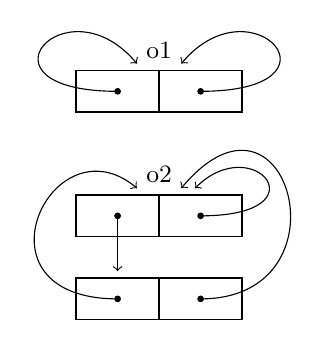
\begin{tikzpicture}
  \clip (-1.75em,-0.25em) rectangle (8.00em, 10.55em);

% o2
  \draw [semithick] (0.0em, 0.0em) rectangle (6.0em, 1.5em);
  \draw [semithick] (3.0em, 0.0em) -- (3.0em, 1.5em);
  \draw [semithick] (0.0em, 3.0em) rectangle (6.0em, 4.5em);
  \draw [semithick] (3.0em, 3.0em) -- (3.0em, 4.5em);

  \draw [->] (1.5em, 0.75em) .. controls +(180:5.5em) and +(140:4.0em) .. (2.2em, 4.75em);
  \draw [->] (4.5em, 0.75em) .. controls +(  0:5.5em) and +( 50:6.0em) .. (3.8em, 4.75em);
  \draw [->] (4.5em, 3.75em) .. controls +(  0:4.5em) and +( 45:3.0em) .. (4.3em, 4.75em);
  \draw [->] (1.5em, 3.75em) -- (1.5em, 1.75em);

  \filldraw  (1.5em, 0.75em) circle(1.0pt);
  \filldraw  (4.5em, 0.75em) circle(1.0pt);
  \filldraw  (1.5em, 3.75em) circle(1.0pt);
  \filldraw  (4.5em, 3.75em) circle(1.0pt);

% o1
  \draw [semithick] (0.0em, 7.5em) rectangle (6.0em, 9.0em);
  \draw [semithick] (3.0em, 7.5em) -- (3.0em, 9.0em);

  \draw [->] (1.5em, 8.25em) .. controls +(180:5.5em) and +(130:4.0em) .. (2.2em, 9.25em);
  \draw [->] (4.5em, 8.25em) .. controls +(  0:5.5em) and +( 50:4.0em) .. (3.8em, 9.25em);

  \filldraw  (1.5em, 8.25em) circle(1.0pt);
  \filldraw  (4.5em, 8.25em) circle(1.0pt);


  \draw (3.0em, 4.6em) node[above] {\small\ic{o2}};
  \draw (3.0em, 9.1em) node[above] {\small\ic{o1}};

\end{tikzpicture}

\ifPreview\else\end{float:right}\fi

% </MAGIC>

\begin{code:lisp}
(define o1 (let ((pair (cons 1 2)))
             (set-car! pair pair)
             (set-cdr! pair pair)
             pair ))
(define o2 (let ((pair (cons (cons 1 2))))
             (set-car! (car pair) pair)
             (set-cdr! (car pair) pair)
             (set-cdr! pair pair)
             pair ))
\end{code:lisp}

Предположим, мы хотим вычислить~\ic{(equal? o1~o1)}. Пусть \ic{equal?}
реализована так, что сначала вызывает \ic{eq?}, и только потом "--- если ей
переданы объекты, которые действительно могут быть не~эквивалентны, "--- она
выполняет долгую структурную проверку. В~таком случае мы сразу~же получаем
ответ~\ic{\#t}. Иначе \ic{equal?} попадает в~бесконечный цикл.%
\footnote*{Я~запускал этот пример на четырёх различных интерпретаторах~Scheme и
два из них зациклились. Я~не~буду их называть, так как у~них есть полное право
так делать. \cite{kcr98}}

Ладно, пусть результат \ic{(equal? o1~o1)} зависит от реализации; что насчёт
\ic{(equal? o1~o2)}? И~опять ответ зависит от того, изменяемы~ли или~нет
точечные пары, из которых состоят \ic{o1} и~\ic{o2}. Если они неизменяемы, то
без \ic{eq?} нельзя написать программу, которая~бы смогла отличить \ic{o1}
от~\ic{o2}. Таким образом, лучше воздержаться от сравнения циклических структур
данных с~помощью~\ic{equal?}.

\bigskip

\indexR{сравнение!символов}
Рассмотренные предикаты поддерживают большую часть используемых типов данных, за
исключением символов и~функций. Символы часто являются не~совсем атомарными,
так как они могут содержать списки свойств. Но с~точки зрения сравнения их можно
считать такими~же неизменяемыми, как и~числа, потому что символ однозначно
определяется своим именем; вся суть символов как раз в~том, что не~может быть
двух различных символов с~одинаковыми именами.

\indexR{списки свойств}
\indexR{символы!списки свойств}
\indexR{хеш-таблицы}
Что касается списков свойств, которые часто хранятся вместе с~символами, то они
являются удобным дополнением, например, для хранения всевозможных метаданных
о~глобальных переменных. В~то~же время, необходимо понимать ответственность за
введение данной возможности: для её поддержки требуются побочные эффекты;
свойства символа доступны глобально; для хранения каждого свойства требуются две
точечные пары; желательно организовать эффективный поиск значения по имени
свойства (например, на основе \term{хеш-таблиц}\footnote{По~моему скромному
мнению, изобретение хеш-таблиц является одним из величайших достижений
информатики.}).


\subsection{Равенство функций}%
\label{assignment/side-effects/ssect:equality-func}

\indexR{сравнение!функций}
\indexR{функции!сравнение}
\indexR{функции!тождественность}
Случай сравнения функций может показаться безнадёжным. Легко догадаться, что
функции эквивалентны, если они дают равные результаты для равных аргументов;
в~таком случае очевидно, что они взаимозаменимы. Более формально
тождественность функций записывается так:
%
\[ f \equals g \iff \forall x \colon f(x) = g(x) \]

К~сожалению, если~бы всё было так просто запрограммировать\textdots\ Мы ведь
не~можем всерьёз проверять все возможные значения аргументов. Поэтому придётся
или отказаться от идеи сравнимости функций, или~же принять менее строгое
определение эквивалентности для них. Сложно сказать, эквивалентны~ли
произвольные функции, но очень часто бывает легко выяснить, когда они
не~эквивалентны (например, если они принимают разное количество аргументов).

Поэтому для функций можно определить приближённое сравнение, понимая при этом,
что оно может ошибаться, порой значительно. Естественно, пользоваться им можно
только в~том случае, если мы точно знаем, когда и насколько его результат будет
ошибочным.

\indexCS{eqv"?}{для функций}
Scheme определяет \ic{eqv?} для функций следующим образом: если есть хотя бы
один набор аргументов, который приводит к~различным результатам применения
функций \ic{f} и~\ic{g}, то данные функции не~эквивалентны. И~снова, здесь речь
идёт о~различии, а не~о~равенстве.

Давайте рассмотрим ещё несколько примеров. Выражение \ic{(eqv? car cdr)} должно
возвращать ложь, так как результаты применения этих функций значительно
отличаются, например, для~\ic{(a~.~b)}.

\indexR{тождественность!функций}
Также очевидно, что \ic{(eqv? car car)} должна возвращать истину, так как
эквивалентность обязана быть рефлексивной. Но в~некоторых реализациях данная
форма возвращает ложь, так как \ic{car} является инлайн-функцией и эта форма
фактически читается как \ic{(eqv? (lambda (x) (car~x)) (lambda (x) (car~x)))}.
{\RnRS} оставляет результат \ic{eqv?} при подобном сравнении на усмотрение
реализации.

А~как сравнить \ic{cons} и \ic{cons}, не~прибегая к~спасительной рефлексивности?
Ведь функция~\ic{cons} создаёт изменяемые структуры данных, так что даже если её
аргументы можно сравнить, то результаты вовсе не~обязаны быть эквивалентными,
так как они размещаются в~разных участках памяти. Таким образом, \ic{cons}
не~тождественна \ic{cons}, и \ic{(eqv? cons~cons)} должна вернуть ложь, так как
\ic{(eqv? (cons~1~2) (cons~1~2))} возвращает ложь!

\indexR{частичные функции}
\indexR{функции!частичные}
Вы всё ещё уверены, что \ic{car} должна быть равна~\ic{car}? Есть и другие
проблемы. Например, в~языке без проверки типов \ic{(car~’foo)} вызовет ошибку и
выброс исключения, но результаты его перехвата и обработки слабо предсказуемы и
зависят отнюдь не~только от аргументов. Поэтому не~все функции вообще могут
вернуть что"~то сравнимое. Это касается всех частичных функций,\trnote*{Функция
$f\colon X \to Y$ называется частичной, если её значения на~$X$ могут быть
не~определены. Классический пример: операция вычитания для натуральных чисел
имеет тип $\mathbb{N} \times \mathbb{N} \to \mathbb{N}$, но определена не~для
всех пар натуральных чисел $(a, b) \in \mathbb{N} \times \mathbb{N}$, только для
тех, где $a \geq b$.} которые используются вне своей фактической области
определения.

\indexR{замыкания (closures)!сравнение}
Так что~же делать? В~различных языках применяются различные меры. Некоторые
языки имеют мощную систему типов, поэтому они в~состоянии определить, когда
аргументы сравнения являются функциями; часть диалектов ML, например, этим
пользуется, запрещая сравнивать функции вообще. В~Scheme форма \ic{lambda}
создаёт замыкания. Каждый вызов \ic{lambda} сохраняет в~памяти замыкание,
которое имеет определённый адрес, так что функции можно сравнивать хотя~бы по
этому адресу. Именно так и делает \ic{eqv?}, считая функции с~одинаковым адресом
эквивалентными.

Однако, такое поведение может мешать некоторым оптимизациям. Рассмотрим функцию
с~говорящим именем \ic{make-named-box}. Она принимает один аргумент (сообщение),
анализирует его и реагирует соответствующим образом. Это один из возможных
способов реализации объектов, именно его мы будем использовать для написания
интерпретатора в~этой главе.

\indexC{make-named-box}
\begin{code:lisp}
(define (make-named-box name value)
  (lambda (msg)
    (case msg
      ((type) (lambda () 'named-box))
      ((name) (lambda () name))
      ((ref)  (lambda () value))
      ((set!) (lambda (new-value) (set! value new-value))) ) ) )
\end{code:lisp}

Замечательно, мы научились привязывать к~коробкам бирку с~именем. Теперь
рассмотрим функцию внимательнее: замыкание, возвращаемое в~ответ на сообщение
\ic{type}, не~зависит от локальных переменных. Поэтому его можно вынести за
скобки:

\begin{code:lisp}
(define other-make-named-box
  (let ((type-closure (lambda () 'named-box)))
    (lambda (name value)
      (let ((name-closure  (lambda () name))
            (value-closure (lambda () value))
            (set!-closure  (lambda (new-value)
                             (set! value new-value) )) )
        (lambda (msg)
          (case msg
            ((type) type-closure)
            ((name) name-closure)
            ((ref)  value-closure)
            ((set!) set!-closure) ) ) ) ) ) )
\end{code:lisp}

\noindent
Отлично, \ic{type-closure} теперь создаётся только один раз для всех коробок, а
не~при каждом разборе~\ic{msg}.

Но что мы получим в~результате следующего сравнения?

\begin{code:lisp}
(let ((box (make-named-box 'foo 33)))
  (|\ii{равны}|? (box 'type) (box 'type)) )
\end{code:lisp}

Это не~совсем корректный вопрос, потому что здесь не~указан предикат. Если это
\ic{eq?}, то ответ зависит от количества созданных копий \ic{(lambda~()
'named-box)}, если~же это~\ic{egal}, то расположение замыканий не~играет роли и
ответом будет истина. Таким образом, семантика языка неявно зависит от
предоставляемых им предикатов сравнения.

Если \ic{lambda} создаёт замыкания в~памяти, то у~них всегда есть какой"~то
адрес. Два замыкания с~одинаковым адресом, очевидно, являются одним и тем~же
замыканием, а потому эквивалентны. Соответственно, в~Scheme следующая программа
ведёт себя верно:

\begin{code:lisp}
(let ((f (lambda (x y) (cons x y))))
  (eqv? f f) ) |\is| #t
\end{code:lisp}

\noindent
Так как \ic{eqv?} передан один и тот~же объект, она вправе вернуть истину; даже
если \ic{(eqv? (f~1~2) (f~1~2))} возвращает ложь.

\bigskip

Как мы видим, при сравнении функций возникает множество вопросов, на которые
нельзя дать однозначный ответ. Предпочтения зависят от свойств эквивалентности,
которые желательно сохранить в~языке, так как проверка математической
тождественности функций не~представляется возможной. Свойства подобного
сравнения зависят от выбора авторов реализации языка. Иногда оно и вообще
оказывается под запретом. Хотя в~этой книге сравнение функций всё~же
используется для методов {\Meroonet} \seePage[objects/method/par:func-eq],
пожалуйста, если это возможно, старайтесь воздержаться от сравнения функций
в~любом~виде.


\section{Реализация}\label{assignment/sect:implementation}

\indexR{обмен сообщениями}
\indexR{замыкания (closures)}
\indexR{сообщения}
В~этот раз мы напишем интерпретатор, основанный на замыканиях. Все его объекты
будут \ic{lambda}-формами, которые отправляют сообщения другим формам и
разбирают входящие сообщения с~помощью уже знакомой вам идиомы \ic{(lambda (msg)
(case msg~...))}. Некоторые сообщения будут универсальными для всех объектов.
Сообщение \ic{boolify} запрашивает у~объекта его булев эквивалент (то~есть
\ic{\#t} или \ic{\#f} для нужд \ic{if}-форм), а сообщение \ic{type}, конечно~же,
вернёт его тип.

Главной проблемой является способ реализации побочных эффектов. Формально,
переменная ссылается на привязку, которая указывает на значение этой переменной.
Говоря простым языком, переменная указывает на коробку (адрес), где лежит
её значение. Память "--- это функция, достающая из нужной коробки значение.
Окружение "--- это функция, достающая из кучи нужную коробку. Всё это просто и
понятно, но ровно до того момента, как мы попытаемся это запрограммировать.

\indexR{вычисления!контекст}
\indexR{контекст вычислений}
Память должна быть видна отовсюду. Можно было~бы сделать её глобальной
переменной, но это не~совсем элегантное решение, ведь вы знаете, сколько проблем
и неоднозначностей таит в~себе глобальное окружение. Есть и другой способ
обеспечить видимость памяти для всех функций интерпретатора: передавать её как
аргумент в~каждую функцию, а она будет передавать её в~следующую (возможно,
изменив перед этим). Так и поступим; теперь вычисление описывается четвёркой из
\term{выражения}, \term{окружения}, \term{продолжения} и~\term{памяти}.
В~программе будем их коротко называть \ic{e}, \ic{r}, \ic{k} и~\ic{s}.

\indexR{соглашения именования}
\indexE{e @\protect\ic{e} (выражения)}
\indexE{r @\protect\ic{r} (лексическое окружение)}
\indexE{k @\protect\ic{k} (продолжения)}
\indexE{v @\protect\ic{v} (значения)}
\indexE{f @\protect\ic{f} (функции)}
\indexE{n @\protect\ic{n} (идентификаторы)}
\indexE{s @\protect\ic{s} (память)}
\indexE{a @\protect\ic{a} (адреса)}
Как обычно, функция \ic{evaluate} проводит синтаксический анализ своего
аргумента и вызывает соответствующую функцию-вычислитель. Не~будем нарушать
установленную в~предыдущих главах традицию именования сущностей, лишь расширим
список новыми типами:

\begin{center}\begin{tabular}{rl}
\ic{e}, \ic{et}, \ic{ec}, \ic{ef} & выражения, формы  \\
                           \ic{r} & окружения         \\
                  \ic{k}, \ic{kk} & продолжения       \\
                \ic{v}, \ic{void} & значения          \\
                           \ic{f} & функции           \\
                           \ic{n} & идентификаторы    \\
        \ic{s}, \ic{ss}, \ic{sss} & память            \\
                  \ic{a}, \ic{aa} & адреса (коробки)
\end{tabular}\end{center}

Так как у~нас увеличилось количество аргументов функций, то отныне будем всегда
их перечислять в~определённом порядке: \ic{e}, \ic{r}, \ic{s}, затем~\ic{k}.

Итак, ядро интерпретатора:

\indexC{evaluate}
\begin{code:lisp}
(define (evaluate e r s k)
  (if (atom? e)
      (if (symbol? e) (evaluate-variable e r s k)
          (evaluate-quote e r s k) )
      (case (car e)
        ((quote)  (evaluate-quote (cadr e) r s k))
        ((if)     (evaluate-if (cadr e) (caddr e) (cadddr e) r s k))
        ((begin)  (evaluate-begin (cdr e) r s k))
        ((set!)   (evaluate-set! (cadr e) (caddr e) r s k))
        ((lambda) (evaluate-lambda (cadr e) (cddr e) r s k))
        (else     (evaluate-application (car e) (cdr e) r s k)) ) ) )
\end{code:lisp}


\subsection{Ветвление}\label{assignment/implementation/ssect:condition}

\ForLayout{display}{\begingroup
\lstset{aboveskip=\smallskipamount, belowskip=\smallskipamount}}

Условный оператор требует вспомогательного продолжения для выполнения ветвления
после вычисления условия.

\indexC{evaluate-if}
\begin{code:lisp}
(define (evaluate-if ec et ef r s k)
  (evaluate ec r s
    (lambda (v ss)
      (evaluate ((v 'boolify) et ef) r ss k) ) ) )
\end{code:lisp}

Вспомогательное продолжение принимает не~только вычисленное условие~\ic{v}, но и
состояние памяти после вычисления. Следовательно, мы допускаем побочные эффекты
при вычислении условия:

\begin{code:lisp}
(if (begin (set-car! pair 'foo)
           (cdr pair) )
    (car pair) 2 ) |{\is} \ic{'foo} \textrm{или} \ic{2}|
\end{code:lisp}

\indexR{поиск с возвратом}
Сейчас любые изменения памяти, выполненные в~условии, видны в~обеих ветках. Но
можно поступить иначе:

\indexCS{evaluate-if}{поиск с возвратом}
\begin{code:lisp}
(define (evaluate-amnesic-if ec et ef r s k)
  (evaluate ec r s
    (lambda (v ss)
      (evaluate ((v 'boolify) et ef) r s     ; $\ic{s} \ne \ic{ss}$!
                k) ) ) )
\end{code:lisp}

В~этом случае при вычислении веток мы пользуемся старым состоянием памяти,
которое было при вызове самой формы~\ic{if}. Это необходимое свойство для языков
со~встроенной поддержкой поиска с~возвратом вроде~Пролога.
\seeEx[assignment/ex:form-or]

\indexE{boolify@\protect\ic{'boolify}}
\indexR{комбинаторы!T@\protect\comb{T}}
\indexR{комбинаторы!F@\protect\comb{F}}
Так как мы решили все объекты интерпретатора представлять функциями, то
в~качестве логических значений нельзя использовать \ic{\#t} и~\ic{\#f} языка
реализации. Кроме этого нам необходим способ приведения любых объектов
к~логическому типу (ведь любой объект в~Scheme, кроме~\ic{\#f}, считается
логической истиной). Будем считать, что все объекты отвечают на сообщение
\ic{boolify}, возвращая своё логическое представление в~виде одного из
комбинаторов $\lambda$"=исчисления: \ic{(lambda (x~y)~x)} или
\ic{(lambda (x~y)~y)}.

\ForLayout{display}{\endgroup}% \lstset *skipamount


\subsection{Последовательность}\label{assignment/implementation/ssect:sequence}

Хотя тут нет ничего интересного или нового, но повторить смысл последовательных
вычислений будет не~лишним. Для простоты мы считаем, что \ic{begin} передана
как минимум одна форма.

\indexC{evaluate-begin}
\begin{code:lisp}
(define (evaluate-begin e* r s k)
  (if (pair? (cdr e*))
      (evaluate (car e*) r s
        (lambda (void ss)
          (evaluate-begin (cdr e*) r ss k) ) )
      (evaluate (car e*) r s k) ) )
\end{code:lisp}

Здесь чётко видно, как мы последовательно вычисляем тело \ic{begin}, передаём
новое состояние памяти, но игнорируем значения всех вычисляемых выражений, кроме
последнего, которое обрабатывается отдельно.


\subsection{Окружения}\label{assignment/implementation/ssect:environment}

Окружения представляются функциями, переводящими имена переменных в~адреса.
Аналогично, память "--- это функция, переводящая адреса в~значения. Начальное
окружение должно быть пустым:

\indexC{r.init}
\begin{code:lisp}
(define (r.init id)
  (wrong "No binding for" id) )
\end{code:lisp}

\indexR{память!чисто функциональная}
\indexR{чисто функциональные структуры данных}
\indexR{побочные эффекты}
Итак, как~же нам выразить изменение окружения (или памяти), не~используя
побочные эффекты или присваивание? В~нашем случае это значит, что функция-память
должна после изменения по-другому реагировать на определённое значение, но
по-старому "--- на все остальные. Функция~\ic{update} создаёт новую память
именно с~таким поведением:

\indexC{update}
\begin{code:lisp}
(define (update s a v)
  (lambda (aa)
    (if (eqv? a aa) v (s aa)) ) )
\end{code:lisp}

Здесь буквально записана эта идея. Вызов \ic{(update s a~v)} вернёт новое,
изменённое состояние памяти, которое мы передадим следующей функции как текущее.
Также можно обобщить \ic{update} для изменения сразу нескольких значений:

\indexC{update*}
\begin{code:lisp}
(define (update* s a* v*)
  ;; \ic{(assume (= (length a*) (length v*)))}
  (if (pair? a*)
      (update* (update s (car a*) (car v*)) (cdr a*) (cdr v*))
      s ) )
\end{code:lisp}

Функция \ic{update} одинаково хорошо работает как с~памятью, так и
с~окружениями. В~ML это была~бы полиморфная функция, так как окружения и память
имеют разные типы. Также необходимо учитывать, что \ic{update} требуется некий
критерий сравнения адресов, поэтому для их представления стоит выбрать
гарантированно сравнимые объекты: например, целые числа. Имена переменных мы
будем представлять символами. Оба типа данных прекрасно поддерживаются
\ic{eqv?}, поэтому в~\ic{update} используется именно этот предикат.


\subsection{Обращения к~переменным}%
\label{assignment/implementation/ssect:reference}

Благодаря выбранному представлению памяти значение переменной получается
элементарно:

\indexC{evaluate-variable}
\begin{code:lisp}
(define (evaluate-variable n r s k)
  (k (s (r n)) s) )
\end{code:lisp}

Сначала мы извлекаем адрес переменной \ic{(r~n)} из окружения, затем ищем
соответствующее значение в~памяти~\ic{s} и передаём его продолжению~\ic{k}. Так
как чтение памяти не~вызывает побочных эффектов, то продолжению память
передаётся в~неизменном виде.


\subsection{Присваивание}\label{assignment/implementation/ssect:assignment}

Для присваивания необходимо промежуточное продолжение.

\indexC{evaluate-set"!}
\begin{code:lisp}
(define (evaluate-set! n e r s k)
  (evaluate e r s
    (lambda (v ss)
      (k v (update ss (r n) v)) ) ) )
\end{code:lisp}

Новое значение переменной после вычисления передаётся продолжению, которое
записывает его в~память по адресу переменной. Дальше промежуточное продолжение
передаёт обновлённое состояние памяти изначальному продолжению формы \ic{set!}.
Между прочим, возвращаемое значение этого варианта присваивания вполне
определено: это текущее значение переменной после присваивания.

Принцип работы памяти без побочных эффектов и причины представления её как
функции теперь должны быть окончательно понятны: фактически, память
представляется историей изменений своего состояния. Мы никогда не~изменяем
записи в~этом списке и не~удаляем их "--- только добавляем новые, переопределяя
таким образом функцию-память. Конечно, если сравнивать его с~реальной памятью,
данный вариант является жутко неэффективным и избыточным, но ведение истории
изменений имеет свои плюсы. \seeEx[assignment/ex:previous-value] По~крайней
мере, можно взять эту идею на вооружение хотя~бы частично.


\subsection{Аппликация}\label{assignment/implementation/ssect:application}

Перед применением функции необходимо вычислить все элементы формы вызова.
Вычислять их можно, как известно, в~произвольном порядке. Пусть это будет
порядок слева направо.

\indexC{evaluate-application}
\begin{code:lisp}
(define (evaluate-application e e* r s k)
  (define (evaluate-arguments e* r s k)
    (if (pair? e*)
        (evaluate (car e*) r s
          (lambda (v ss)
            (evaluate-arguments (cdr e*) r ss
              (lambda (v* sss)
                (k (cons v v*) sss) ) ) ) )
        (k '() s) ) )
  (evaluate e r s
    (lambda (f ss)
      (evaluate-arguments e* r ss
        (lambda (v* sss)
          (if (eq? (f 'type) 'function)
              ((f 'behavior) v* sss k)
              (wrong "Not a function" f) ) ) ) ) ) )
\end{code:lisp}

\indexE{behavior@\protect\ic{'behavior}}
Здесь функция, которая обычно называлась \ic{evlis}, является локальной и
называется \ic{evaluate-arguments}. Она вычисляет аргументы слева направо и
собирает их в~список. Затем функция (первый элемент формы) применяется
к~аргументам вместе с~памятью после их вычисления и продолжением вызова функции.
Обратите внимание на то, как лаконично и точно записаны эти идеи.

Функции представляются специальными замыканиями, так что напрямую их применять
нельзя. Поэтому вводится сообщение \ic{behavior} для извлечения поведения
функции: кода, который будет применён к~аргументам.


\subsection{Абстракция}\label{assignment/implementation/ssect:abstraction}

\indexCS{lambda}{и~память}
Для простоты будем считать, что специальная форма \ic{lambda} поддерживает
только функции с~фиксированным количеством аргументов. При создании функции
происходит две вещи: в~памяти выделяется ячейка, затем создаётся особый объект
"--- замыкание, "--- которое и размещается в~только что выделенной ячейке
памяти. Очевидно, что созданную функцию надо где"~то хранить для дальнейшего
использования, поэтому форма \ic{lambda} вынуждена изменять состояние памяти.
Работа по созданию и сохранению замыканий перекладывается на функцию
\ic{create-function}, которой передаётся адрес выделенного участка памяти и код
функции "--- именно тот, который должно вернуть замыкание в~ответ на сообщение
\ic{behavior}.

\indexC{evaluate-lambda}
\begin{code:lisp}
(define (evaluate-lambda n* e* r s k)
  (allocate 1 s
    (lambda (a* ss)
      (k (create-function
          (car a*)
          (lambda (v* s k)
            (if (= (length n*) (length v*))
                (allocate (length n*) s
                  (lambda (a* ss)
                    (evaluate-begin e*
                                    (update* r  n* a*)
                                    (update* ss a* v*)
                                    k ) ) )
                (wrong "Incorrect arity") ) ) )
          ss ) ) ) )
\end{code:lisp}

При вызове функции, созданной \ic{lambda}, сначала проверяется количество
переданных аргументов, затем в~памяти в~момент вызова выделяется место для
аргументов функции, после чего они инициализируются переданными значениями и,
наконец, управление передаётся собственно функции.

\indexR{функции!в~Фортране}
Возможен и другой вариант реализации:

\begin{code:lisp}
(define (evaluate-ftn-lambda n* e* r s k)
  (allocate (+ 1 (length n*)) s
    (lambda (a* ss)
      (k (create-function
          (car a*)
          (lambda (v* s k)
            (if (= (length n*) (length v*))
                (evaluate-begin e*
                                (update* r n* (cdr a*))
                                (update* s (cdr a*) v*)
                                k )
                (wrong "Incorrect arity") ) ) )
      ss ) ) ) )
\end{code:lisp}

\noindent
В~этом случае место в~памяти под аргументы выделяется один раз при создании
замыкания; так поступает, например, Фортран. Но, к~сожалению, такой подход
лишает нас рекурсии, ведь теперь нет возможности хранить несколько отдельных
наборов аргументов для каждого вызова функции. В~Фортране подобное решение
принято по той причине, что раз там нет динамического создания функций, то
память для аргументов можно выделить ещё при компиляции, что приводит к~росту
производительности. Правда, ценой рекурсии и замыканий "--- главных достоинств
функциональных языков.


\subsection{Память}\label{assignment/implementation/ssect:memory}

\indexR{сборка мусора}
Память представляется функцией, принимающей адреса и возвращающей значения.
Кроме этого нам нужна возможность выделять в~памяти новые адреса, гарантированно
свободные для использования; этим будет заниматься функция~\ic{allocate}. Она
принимает три аргумента: необходимое количество адресов, память и продолжение,
которому она передаст список выделенных адресов и новое состояние памяти, где по
соответствующим адресам хранятся значения <<не~инициализировано>>. Именно на эту
функцию возложена вся работа по управлению памятью, в~частности, сборка мусора.
Это отдельная сложная тема,\trnote*{Достаточно неплохое введение в~сборку мусора
есть в~первом томе <<Искусства программирования>> Дональда~Кнута.} которой мы
не~будем здесь касаться и предположим, что память у~нас бесконечная "---
то~есть мы всегда можем найти необходимое количество свободных адресов.

\indexC{allocate}
\begin{code:lisp}
(define (allocate n s k)
  (if (> n 0)
      (let ((a (new-location s)))
        (allocate (- n 1)
                  (expand-store a s)
                  (lambda (a* ss)
                    (k (cons a a*) ss) ) ) )
      (k '() s) ) )
\end{code:lisp}

Функция \ic{new-location} ищет первый свободный адрес в~памяти. Это настоящая
чистая функция в~том смысле, что \ic{(eqv? (new-location~s) (new-location~s))}
всегда возвращает истину. Если выделять ячейки в~памяти последовательно, то
достаточно будет хранить последний выделенный адрес для определения следующего
свободного. Резервируется ячейка памяти с~помощью функции \ic{expand-store}.

\indexC{expand-store}
\indexC{new-location}
\begin{code:lisp}
(define (expand-store high-location s)
  (update s 0 high-location) )

(define (new-location s)
  (+ 1 (s 0) ) )
\end{code:lisp}

Как видим, адрес последней выделенной ячейки сам хранится в~памяти по адресу~0.
Память отзывается на два типа сообщений: запрос адреса свободной ячейки (при
передаче нуля) и запрос значения по адресу (при передаче иных адресов). Это
просто и удобно для реализации. Естественно, также необходимо определить
изначальное состояние памяти, где не~выделено ни~одной ячейки:

\indexC{s.init}
\begin{code:lisp}
(define s.init
  (expand-store 0 (lambda (a) (wrong "No such address" a))) )
\end{code:lisp}


\subsection{Представление значений}%
\label{assignment/implementation/ssect:values}

Мы решили представлять данные внутри интерпретатора в~виде замыканий,
обменивающихся сообщениями. Для простоты ограничимся пустым списком, булевыми
значениями, символами, числами, точечными парами и~функциями. Рассмотрим эти
типы данных по~очереди.

\indexE{type@\protect\ic{'type}}
\indexE{boolify@\protect\ic{'boolify}}
Все значения будут основываться на функции, которая отвечает как минимум на два
сообщения: 1)~запрос типа (\ic{type}); 2)~приведение к~логическому типу
(\ic{boolify}). Значения конкретных типов данных будут реагировать на свои
специфичные сообщения. Таким образом, все определения значений имеют следующий
скелет:

\begin{code:lisp}
(lambda (msg)
  (case msg
    ((type)    ...)
    ((boolify) ...)
    ... ) )
\end{code:lisp}

Существует только один пустой список и, в~соответствии с~\RnRS, для \ic{if} он
является истиной.

\indexC{the-empty-list}
\begin{code:lisp}
(define the-empty-list
  (lambda (msg)
    (case msg
      ((type)    'null)
      ((boolify) (lambda (x y) x)) ) ) )
\end{code:lisp}

Булевы значения создаются функцией \ic{create-boolean}:

\indexC{create-boolean}
\begin{code:lisp}
(define (create-boolean value)
  (let ((combinator (if value (lambda (x y) x)
                              (lambda (x y) y) )))
    (lambda (msg)
      (case msg
        ((type)    'boolean)
        ((boolify) combinator) ) ) ) )
\end{code:lisp}

\indexE{name@\protect\ic{'name}}
Символы имеют имя, которое они назовут, если их вежливо попросить с~помощью
\ic{name}. Мы будем представлять их имена родными символами Scheme.

\indexC{create-symbol}
\begin{code:lisp}
(define (create-symbol v)
  (lambda (msg)
    (case msg
      ((type)    'symbol)
      ((name)    v)
      ((boolify) (lambda (x y) x)) ) ) )
\end{code:lisp}

\indexE{value@\protect\ic{'value}}
Числа~же будут отвечать на сообщение~\ic{value}:

\indexC{create-number}
\begin{code:lisp}
(define (create-number v)
  (lambda (msg)
    (case msg
      ((type)    'number)
      ((value)    v)
      ((boolify) (lambda (x y) x)) ) ) )
\end{code:lisp}

\indexE{behavior@\protect\ic{'behavior}}
\indexE{tag@\protect\ic{'tag}}
Функции имеют более развитый словарный запас из двух сообщений: \ic{tag}
и~\ic{behavior}. Сообщение \ic{behavior}, конечно~же, вернёт код функции;
\ic{tag} хранит адрес, по~которому эта функция расположена в~памяти.

\indexC{create-function}
\begin{code:lisp}
(define (create-function tag behavior)
  (lambda (msg)
    (case msg
      ((type)     'function)
      ((boolify)  (lambda (x y) x))
      ((tag)      tag)
      ((behavior) behavior) ) ) )
\end{code:lisp}

\indexR{точечные пары!представление}
\indexR{представление!точечных пар}
\indexC{cdr}
Остались только точечные пары. Точечная пара "--- это объект, состоящий из
двух значений, каждое из которых можно изменять независимо. Поэтому мы будем их
представлять в~виде двух адресов: один будет ссылаться на~\ic{car}, второй "---
на~\ic{cdr}. Это может показаться необычным, так как традиционно точечные пары
представляются не~двумя отдельными коробками, а одной коробкой с~двумя
отделениями.\footnote*{Причём по~результатам серьёзных исследований
вроде~\cite{cla79,cg77}, желательно, чтобы значение \ic{cdr} (а~не~\ic{car}),
было доступно непосредственно. Другим преимуществом такого расположения может
быть то, что точечные пары используются для представления связных списков,
поэтому можно ввести общий класс <<связных~объектов>> с~единственным
полем~\ic{cdr}.} Это~бы позволило чуть быстрее обращаться к~её компонентам, а
также применить известную технику размещения точечных пар в~параллельных
массивах: хранить \ic{car} и \ic{cdr} пар в~двух отдельных массивах, но по
одинаковым индексам; тогда адресом пары будет именно этот индекс. Но мы
останемся верны идее привязок и будем хранить пары в~виде двух адресов.

Для удобства мы также введём функцию, выделяющую в~памяти целые списки. Она
принимает список значений, которые необходимо разместить в~памяти, собственно
память и продолжение, которому эта функция передаст созданный список и новое
состояние памяти.

\indexC{allocate-list}
\indexC{allocate-pair}
\indexC{create-pair}
\begin{code:lisp}
(define (allocate-list v* s k)
  (define (consify v* k)
    (if (pair? v*)
        (consify (cdr v*) (lambda (v ss)
                            (allocate-pair (car v*) v ss k) ))
        (k the-empty-list s) ) )
  (consify v* k) )

(define (allocate-pair a d s k)
  (allocate 2 s
   (lambda (a* ss)
     (k (create-pair (car a*) (cadr a*))
        (update (update ss (car a*) a) (cadr a*) d) ) ) ) )

(define (create-pair a d)
  (lambda (msg)
    (case msg
      ((type)    'pair)
      ((boolify) (lambda (x y) x))
      ((set-car) (lambda (s v) (update s a v)))
      ((set-cdr) (lambda (s v) (update s d v)))
      ((car)     a)
      ((cdr)     d) ) ) )
\end{code:lisp}


\subsection{Сравнение с~объектным~подходом}%
\label{assignment/implementation/ssect:cmp-to-oop}

\indexR{замыкания (closures)!и объекты}
\indexR{объекты!как замыкания}
Замыкания, реагирующие на сообщения, с~помощью которых мы представляем значения
внутри интерпретатора, во~многом напоминают объекты из предыдущей главы. Тем
не~менее, между подобными объектами"=замыканиями и объектами {\Meroonet} есть
ряд отличий. Объекты"=замыкания хранят поддерживаемые методы внутри; нет
возможности добавлять однажды созданным объектам новые методы. Понятия классов
и подклассов здесь присутствуют лишь умозрительно. В~то~же время, обобщённые
функции позволяют расширять поведение объектов в~любое время и в~любом месте.
С~помощью обобщённых функций можно реализовать как методы, так и мультиметоды.
Объекты из предыдущей главы поддерживают наследование, что позволяет выносить
общие свойства в~базовые классы, избегая дублирования кода. Поэтому не~стоит
думать об~объектах как о~<<замыканиях для бедных>>, как считают некоторые
фанатики Scheme, ведь даже объекты из предыдущей главы оказались значительно
выразительнее. Хотя это не~значит, что замыкания ни~на~что не~способны
\cite{ar88}.


\subsection{Начальное окружение}\label{assignment/implementation/ssect:init-env}

Как обычно, мы определим два вспомогательных макроса, которые помогут создать
начальное окружение (а~также состояние памяти). Под каждую глобальную переменную
необходимо выделить ячейку памяти, адрес которой будет храниться в~глобальном
окружении. Макрос \ic{definitial} выделяет память и кладёт туда указанное
значение.

\indexC{s.global}
\indexC{r.global}
\indexC{definitial}
\begin{code:lisp}
(define s.global s.init)
(define r.global r.init)
|\ForLayout{display}{\vskip-0.4\baselineskip}|
(define-syntax definitial
  (syntax-rules ()
   ((definitial name value)
    (allocate 1 s.global
     (lambda (a* ss)
       (set! r.global (update r.global 'name (car a*)))
       (set! s.global (update ss (car a*) value)) ) ) ) ) )
\end{code:lisp}

\noindent
Макрос \ic{defprimitive} определяет глобальные функции.

\indexC{defprimitive}
\begin{code:lisp}
(define-syntax defprimitive
  (syntax-rules ()
   ((defprimitive name value arity)
    (definitial name
     (allocate 1
      s.global
      (lambda (a* ss)
        (set! s.global (expand-store (car a*) ss))
        (create-function (car a*)
         (lambda (v* s k)
           (if (= arity (length v*))
               (value v* s k)
               (wrong "Incorrect arity" 'name ) )) ) ) ) ) ) ) )
\end{code:lisp}

По уже сложившейся традиции, определим глобальные переменные для истины, лжи
и~пустого списка:

\begin{code:lisp}
(definitial t (create-boolean #t))
(definitial f (create-boolean #f))
(definitial nil the-empty-list)
\end{code:lisp}

В~качестве примера определения примитивов покажем предикат и арифметическую
операцию. Они проверяют типы аргументов, извлекают значения, выполняют
соответствующие действия и упаковывают результат во~внутреннее представление.

\begin{code:lisp}
(defprimitive <=
  (lambda (v* s k)
    (if (and (eq? ((car v*)  'type) 'number)
             (eq? ((cadr v*) 'type) 'number) )
        (k (create-boolean (<= ((car v*) 'value)
                               ((cadr v*) 'value) )) s)
        (wrong "Numbers required" '<=) ) )
  2 )
|\ForLayout{display}{\vskip-0.5\baselineskip}|
(defprimitive *
  (lambda (v* s k)
    (if (and (eq? ((car v*)  'type) 'number)
             (eq? ((cadr v*) 'type) 'number) )
        (k (create-number (* ((car v*) 'value)
                             ((cadr v*) 'value) )) s)
        (wrong "Numbers required" '*) ) )
  2 )
\end{code:lisp}


\subsection{Точечные пары}\label{assignment/implementation/ssect:dotted-pairs}

Впервые точечные пары внутри нашего интерпретатора Scheme не~представляются
родными точечными парами Scheme, на котором он написан.

Так как у~нас есть функция~\ic{allocate-pair}, то определить \ic{cons}
легко:

\ForLayout{display}{\begingroup
\lstset{aboveskip=\smallskipamount, belowskip=\smallskipamount}}

\indexC{cons}
\begin{code:lisp}
(defprimitive cons
  (lambda (v* s k)
    (allocate-pair (car v*) (cadr v*) s k) )
  2 )
\end{code:lisp}

\noindent
С~чтением и модификацией тоже нет~проблем:

\indexC{car}
\indexC{set-cdr"!}
\begin{code:lisp}
(defprimitive car
  (lambda (v* s k)
    (if (eq? ((car v*) 'type) 'pair)
        (k (s ((car v*) 'car)) s)
        (wrong "Not a pair" (car v*)) ) )
  1 )
|\ForLayout{display}{\vskip-0.5\baselineskip}|
(defprimitive set-cdr!
  (lambda (v* s k)
    (if (eq? ((car v*) 'type) 'pair)
        (let ((pair (car v*)))
          (k pair ((pair 'set-cdr) s (cadr v*))) )
        (wrong "Not a pair" (car v*)) ) )
  2 )
\end{code:lisp}

Все значения представляются таким образом, что узнать их тип не~составляет труда
"--- достаточно передать объекту сообщение \ic{type}. Поэтому написать предикат
\ic{pair?} тоже просто, надо только не~забыть перевести результат сравнения
во~внутреннее представление.

\indexC{pair"?}
\begin{code:lisp}
(defprimitive pair?
  (lambda (v* s k)
    (k (create-boolean (eq? ((car v*) 'type) 'pair)) s) )
  1 )
\end{code:lisp}

\ForLayout{display}{\endgroup}% \lstset *skipamount

\subsection{Функция сравнения}%
\label{assignment/implementation/ssect:comparisons}

Одной из задач данного интерпретатора является иллюстрация реализации предиката
эквивалентности "--- \ic{eqv?}. Он проверяет, являются~ли два объекта
взаимозаменимыми. Сначала он сравнивает типы объектов, затем, если они
совпадают, он проводит собственно сравнение. Символы должны иметь одинаковое
имя. Логические значения и числа должны быть одинаковыми. Точечные пары и
функции должны иметь одинаковые адреса.

\indexCS{eqv"?}{реализация}
\begin{code:lisp}
(defprimitive eqv?
  (lambda (v* s k)
    (k (create-boolean
        (if (eq? ((car v*) 'type) ((cadr v*) 'type))
            (case ((car v*) 'type)
              ((null) #t)
              ((boolean)
               (((car v*) 'boolify)
                (((cadr v*) 'boolify) #t #f)
                (((cadr v*) 'boolify) #f #t) ) )
              ((pair)
               (and (= ((car v*) 'car) ((cadr v*) 'car))
                    (= ((car v*) 'cdr) ((cadr v*) 'cdr)) ) )
              ((symbol)
               (eq? ((car v*) 'name) ((cadr v*) 'name)) )
              ((number)
               (= ((car v*) 'value) ((cadr v*) 'value)) )
              ((function)
               (= ((car v*) 'tag) ((cadr v*) 'tag)) )
              (else #f) )
            #f ) )
       s ) )
  2 )
\end{code:lisp}

Собственно, единственная причина, по которой мы сохраняем адреса функций
(а~точнее, замыканий) внутри объектов "--- это сравнение функций с~помощью
\ic{eqv?}. Таким образом, вместо решения сложной проблемы эквивалентности
функций достаточно ответить на простой вопрос о~равенстве адресов, которые суть
просто числа. Заметьте, что при сравнении точечных пар мы тоже сравниваем лишь
адреса компонент, а не~их~содержимое. Итого, \ic{eqv?} выполняется за
предсказуемое постоянное время, в~отличие от~\ic{equal?}.

Функция \ic{eqv?} похожа на обобщённую, только она содержит все методы внутри,
а в~остальном "--- всё та~же диспетчеризация по типу аргумента. Благодаря
выбранному представлению данных мы можем быстро провести проверку на
согласованность типов и перейти непосредственно к~сравнению значений или
адресов, которое чаще всего тоже выполняется быстро (длинной арифметике
не~повезло).


\subsection{Запускаем интерпретатор}%
\label{assignment/implementation/ssect:starting}

Наконец, всё готово для запуска нашего интерпретатора. Главный цикл вызывает
\ic{evaluate} с~рекурсивным продолжением, которое обеспечивает непрерывность
сознания интерпретатора, передавая следующему вызову память предыдущего.

\indexC{chapter4-interpreter}
\begin{code:lisp}
(define (chapter4-interpreter)
  (define (toplevel s)
    (evaluate (read) r.global s
              (lambda (v ss)
                (display (transcode-back v ss))
                (toplevel ss) ) ) )
  (toplevel s.global) )
\end{code:lisp}

\indexR{представление!значений}
Главной особенностью данного интерпретатора является отличие представления
данных интерпретируемого языка от представления данных в~языке реализации.
Особенно разительно отличаются точечные пары и, следовательно, списки, поэтому
мы вынуждены воспользоваться функцией \ic{transcode-back} для преобразования
результата вычислений в~нечто понятное \ic{display}, чтобы его можно было
вывести на экран. Эту вспомогательную функцию вполне можно сразу объединить
с~примитивом \ic{display}.

\indexC{transcode-back}
\begin{code:lisp}
(define (transcode-back v s)
  (case (v 'type)
    ((null)     '())
    ((boolean)  ((v 'boolify) #t #f))
    ((symbol)   (v 'name))
    ((number)   (v 'value))
    ((pair)     (cons (transcode-back (s (v 'car)) s)
                      (transcode-back (s (v 'cdr)) s) ))
    ((function) v)  ; почему бы и нет?
    (else       (wrong "Unknown type" (v 'type))) ) )
\end{code:lisp}


\section{Ввод"~вывод и~память}\label{assignment/sect:io-and-memory}

\indexR{потоки ввода-вывода}
Теперь поговорим о~вводе-выводе. Если ограничиться одним потоком ввода и одним
потоком вывода (то~есть функциями \ic{display} и \ic{read}), то достаточно
добавить каждой функции интерпретатора ещё два аргумента и передавать через них
эти потоки. Поток ввода содержит всё, что программа может прочитать, а поток
вывода содержит всё, что она туда написала. Можно даже предположить, что эти
потоки являются единственным средством связи программы с~внешним миром.

Поток вывода можно легко представить списком пар (\ii{память}, \ii{значение}),
которые передаются функции \ic{transcode-back}. Но как представить поток ввода?
Хитрость здесь в~том, что мы можем вводить и точечные пары со~списками, а они
не~могут существовать отдельно от памяти. Поэтому очевидно, что в~случае чтения
точечных пар необходимо сохранять в~памяти их компоненты. Переводчиком будет
служить функция \ic{transcode}, которая принимает значение языка реализации
(обозначим его~\ic{c}), память и~продолжение. Она переводит это значение
в~представление реализуемого языка и передаёт его продолжению вместе с~новым
состоянием памяти.

\indexC{transcode}
\begin{code:lisp}
(define (transcode c s k)
  (cond
    ((null? c)    (k the-empty-list s))
    ((boolean? c) (k (create-boolean c) s))
    ((symbol? c)  (k (create-symbol c) s))
    ((number? c)  (k (create-number c) s))
    ((pair? c)
     (transcode (car c)
                s
                (lambda (a ss)
                  (transcode (cdr c)
                             ss
                             (lambda (d sss)
                               (allocate-pair a d sss k) ) ) ) ) )
    (else (wrong "Not supported" c)) ) )
\end{code:lisp}

На этом мы остановимся, так как дальнейшая реализация слишком объёмна, чтобы
приводить её здесь полностью: помимо примитивов \ic{read} и~\ic{display},
необходимо в~каждой функции, которую мы написали до этого, расширить набор
аргументов \ic{e}, \ic{r}, \ic{s}, \ic{k} ещё двумя: \ic{i} и~\ic{o}, через
которые и передавать потоки ввода-вывода подобно памяти (потому что они, как и
память, должны быть доступны отовсюду).


\section{Семантика цитирования}\label{assignment/sect:quotation}

\indexR{семантика!цитирования}
Наверное, вы уже заметили, что в~этот раз мы как"~то обошли стороной
цитирование. Форма \ic{quote} раньше всегда записывалась элементарно, но только
потому, что представление значений в~интерпретируемом языке совпадало
с~представлением значений в~самом интерпретаторе. Теперь это не~так, поэтому
определять \ic{quote} следующим образом нельзя:

\begin{code:lisp}
(define (evaluate-quote v r s k)  |\dialect{Ошибка!}|
  (k v s) )
\end{code:lisp}

Здесь ошибочно считается, что \ic{v} "--- это именно то значение, которое
необходимо вернуть. В~смысле, конечно, это именно то, что надо, но это значение
записано на языке, которого наш интерпретатор не~понимает. В~предыдущих главах
интерпретатор пользовался языком реализации, но теперь ему необходим переводчик
"--- \ic{transcode}. Поэтому (более"~менее) правильное определение цитирования
выглядит~так:

\indexC{evaluate-quote}
\begin{code:lisp}
(define (evaluate-quote c r s k)
  (transcode c s k) )
\end{code:lisp}

\indexR{цитаты!композициональность}
\indexR{композициональность!цитат}
Такое определение цитирования \term{композиционально} "--- его смысл зависит
только от аргумента~\ic{c}, оно не~учитывает контекст (значения других
переменных). Но, к~сожалению, точный смысл таких цитат немного отличается от
того, который обычно подразумевается в~Лиспе и~Scheme. Рассмотрим выражение
\ic{(quote (a~.~b))}. По~определению оно \emph{в~точности} эквивалентно
\ic{(cons 'a~'b)}.\footnote*{Ещё точнее: \ic{'(a~.~b) {\equals} `(,'a~.~,'b)}.}
Когда мы цитируем составной объект вроде точечной пары \ic{(a~.~b)}, мы создаём
новую пару в~памяти. Таким образом, такое цитирование "--- это лишь краткая
запись для наших \ic{create-}функций. Поэтому ничуть не~удивительно, что
следующее выражение возвращает ложь:

\begin{code:lisp}
(let ((foo (lambda () '(f o o))))
  (eq? (foo) (foo)) )
\end{code:lisp}

\indexR{эквивалентность!цитат}
\indexR{цитаты!эквивалентность}
\indexR{мемоизация!цитат}
Функция \ic{foo} каждый раз создаёт новый список; все создаваемые значения
независимы, различны в~смысле~\ic{eq?}. Если мы хотим, чтобы данное выражение
всегда возвращало истину, нам необходимо доработать \ic{evaluate-quote} так,
чтобы она возвращала идентичные значения, а не~эквивалентные; для этого она
должна запоминать всё, что возвращала ранее. Это называется \term{мемоизация}.
Одной из причин желательности такого поведения является то, что если в~языке нет
побочных эффектов и \ic{eq?}, то нельзя отличить идентичные объекты от просто
эквивалентных, поэтому нет никакого смысла тратить память на бесполезные копии
эквивалентных объектов, когда можно обойтись одним экземпляром.

Конечно, если допускать побочные эффекты, то дело меняется, но всё~же обычно
считается, что цитаты уникальны "--- как числа, символы и логические значения.

\indexC{evaluate-memo-quote}
\indexC*{shared-memo-quotations}{*shared-memo-quotations*}
\begin{code:lisp}
(define *shared-memo-quotations* '())
(define evaluate-memo-quote
  (lambda (c r s k)
    (let ((couple (assoc c *shared-memo-quotations*)))
      (if (pair? couple)
          (k (cdr couple) s)
          (transcode c s (lambda (v ss)
                           (set! *shared-memo-quotations*
                                 (cons (cons c v)
                                       *shared-memo-quotations* ) )
                           (k v ss) )) ) ) ) )
\end{code:lisp}

\phantomlabel{assignment/quotation/par:transform}
\indexR{преобразование!перенос цитат}
Однако, такой вариант, во-первых, требует побочных эффектов и глобальной
переменной, чего хотелось~бы избежать, а во-вторых, учёт используемых цитат
вполне можно выполнить и заранее, за что компилятор скажет нам спасибо: сначала
мы переносим вычисление цитат в~самое начало программы, затем заменяем все
обращения к~цитатам ссылками на переменные, хранящие вычисленные ранее значения.
На~предыдущем примере это выглядит~так:

{\def\T{\hbox to 0pt{$\leadsto$}}
\begin{code:lisp}
(let ((foo (lambda () '(f o o))))    (define quote35 '(f o o))
  (eq? (foo) (foo)) )             |\T|   (let ((foo (lambda () quote35)))
                                       (eq? (foo) (foo)) )
\end{code:lisp}}

В~итоге цитаты обретают должный смысл, а \ic{evaluate-quote} остаётся такой~же
простой.

Можно было~бы пойти и дальше, полностью избавившись от неоднозначностей,
связанных с~цитированием составных объектов, сделав их создание явным:

\ForLayout{display}{\begingroup
\lstset{aboveskip=\smallskipamount, belowskip=\smallskipamount}}

\begin{code:lisp}
(define quote36 (cons 'o '())
(define quote37 (cons 'o quote36)
(define quote38 (cons 'f quote37)
|\ForLayout{display}{\vskip-0.333\baselineskip}|
(let ((foo (lambda () quote38)))
  (eq? (foo) (foo)) )
\end{code:lisp}

И~ещё дальше, на всякий случай гарантируя правильное цитирование символов
вручную:

\begin{code:lisp}
(define symbol39 (string->symbol "o"))
(define symbol40 (string->symbol "f"))
|\ForLayout{display}{\vskip-0.333\baselineskip}|
(define quote36 (cons symbol39 '())
(define quote37 (cons symbol39 quote36)
(define quote38 (cons symbol40 quote37)
|\ForLayout{display}{\vskip-0.333\baselineskip}|
(let ((foo (lambda () quote38)))
  (eq? (foo) (foo)) )
\end{code:lisp}

Пожалуй, на этом остановимся. На языке ассемблера или Си строки можно
представлять непосредственно, так что было~бы глупо разбивать их на отдельные
символы "--- а~то так ведь можно и до элементарных частиц дойти!

В~конце концов, композициональное определение цитирования оказывается
приемлемым, так как имеет простую формулировку, которая хоть и отличается по
смыслу от традиционного понимания цитирования, но это легко поправимо простым
дополнительным преобразованием программ.

\indexR{гомоиконичность}
Однако, унифицированное представление кода и данных может сыграть с~нами злую
шутку. С~одной стороны это удобно: читать и~данные, и~программы с~помощью одной
функции \ic{read}. Для того, чтобы она могла отличить формы-данные от
форм-программ, как раз и существует специальная форма~\ic{quote}. Но в~том"~то
и дело, что после \ic{quote} данные становятся частью программы. Рассмотрим
пример:

\ForLayout{display}{\endgroup}

\indexC{vowel<=}
\begin{code:lisp}
(define vowel<=
  (let ((vowels '(#\a #\e #\i #\o #\u)))
    (lambda (c1 c2)
      (memq c2 (memq c1 vowels)) ) ) )
|\ForLayout{display}{\vskip-\baselineskip}|
(set-cdr! (vowel<= #\a #\e) '())
(vowel<= #\o #\u) |\is| |\ii{?}|
\end{code:lisp}

При интерпретации этой программы есть высокая вероятность получить не~\ic{\#t},
а~ошибку. И~если после этого мы распечатаем определение \ic{vowel<=} (или
если~бы \ic{vowels} была глобальной), то увидим следующее:

\begin{code:lisp}
(define vowel1<=
  (let ((vowels '(#\a #\e)))
    (lambda (c1 c2)
      (memq c2 (memq c1 vowels)) ) ) )
\end{code:lisp}

\indexR{свёртка констант}
\indexR{константы}
Ой, мы нечаянно кусок программы! Аналогично можно добавлять элементы в~список
\ic{vowels} или изменять их. Правда, такие трюки можно проделывать только
в~интерпретаторе; в~случае компилятора мы скорее всего получим ошибку. Дело
в~том, что если глобальная переменная \ic{vowel<=} неизменяема, то все формы
вроде \ic{(vowel<= \#\bslash a \#\bslash e)} могут быть вычислены ещё на
этапе компиляции, чем компилятор и пользуется, подставляя вместо них сразу
готовый результат. Такая оптимизация называется \term{свёрткой констант}
(\english{constant folding}), её обобщением является техника частичных
вычислений \cite{jgs93}.

Компилятор также может решить подставить константы и в~само определение функции
\ic{vowel<=} ради небольшого ускорения:

\begin{code:lisp}
(define vowel2<=
  (lambda (c1 c2)
    (case c1
      ((#\a) (memq c2 '(#\a #\e #\i #\o #\u)))
      ((#\e) (memq c2 '(#\e #\i #\o #\u)))
      ((#\i) (memq c2 '(#\i #\o #\u)))
      ((#\o) (memq c2 '(#\o #\u)))
      ((#\u) (eq? c2 #\u))
      (else  #f) ) ) )
\end{code:lisp}

\indexR{склеивание цитат}
\indexR{цитаты!склеивание}
Теперь выражение \ic{(eq? (cdr (vowel<= \#\bslash a \#\bslash e)) (vowel<=
\#\bslash e \#\bslash i))} имеет неопределённое значение. С~одной стороны,
оно не~должно быть истиной, так как сравниваемые значения принадлежат явно
различным цитатам. С~другой стороны, иногда оно всё~же истинно: компиляторы
часто оставляют за собой право оптимизировать расположение констант в~памяти,
накладывая их друг на друга и превращая исходную программу в~следующую:

\begin{code:lisp}
(define quote82 (cons #\u '()))
(define quote81 (cons #\o quote82))
(define quote80 (cons #\i quote81)
(define quote79 (cons #\e quote80)
(define quote78 (cons #\a quote79)

(define vowel3<=
  (lambda (c1 c2)
    (case c1
      ((#\a) (memq c2 quote78))
      ((#\e) (memq c2 quote79))
      ((#\i) (memq c2 quote80))
      ((#\o) (memq c2 quote81))
      ((#\u) (eq? c2 #\u))
      (else  #f) ) ) )
\end{code:lisp}

\indexR{константы}
\indexR{связывание!неизменяемое}
Такая оптимизация влияет на разделяемые цитаты и ломает~\ic{eq?}. Есть простой
способ избежать всех этих проблем: запретить изменять цитаты. Именно так и
поступают Scheme и~{\CommonLisp}. Но они делают это мягко, в~общем случае считая
результат изменения значения цитаты неопределённым.

Можно поступить более жёстко, запретив изменение цитат синтаксически:

\indexC{evaluate-immutable-quote}
\indexC{immutable-transcode}
\indexC{allocate-immutable-pair}
\indexC{create-immutable-pair}
\begin{code:lisp}
(define (evaluate-immutable-quote c r s k)
  (immutable-transcode c s k) )

(define (immutable-transcode c s k)
  (cond
    ((null? c)    (k the-empty-list s))
    ((pair? c)
     (immutable-transcode
      (car c) s (lambda (a ss)
                  (immutable-transcode
                   (cdr c) ss (lambda (d sss)
                                (allocate-immutable-pair
                                 a d sss k ) ) ) ) ) )
    ((boolean? c) (k (create-boolean c) s))
    ((symbol? c)  (k (create-symbol c) s))
    ((number? c)  (k (create-number c) s))
    (else (wrong "Not supported" c)) ) )

(define (allocate-immutable-pair a d s k)
  (allocate 2 s
   (lambda (a* ss)
     (k (create-immutable-pair (car a*) (cadr a*))
        (update (update ss (car a*) a) (cadr a*) d) ) ) ) )

(define (create-immutable-pair a d)
  (lambda (msg)
    (case msg
      ((type)    'pair)
      ((boolify) (lambda (x y) x))
      ((set-car) (lambda (s v) (wrong "Immutable pair")))
      ((set-cdr) (lambda (s v) (wrong "Immutable pair")))
      ((car)     a)
      ((cdr)     d) ) ) )
\end{code:lisp}

В~таком случае любая попытка модифицировать цитату обречена на провал. Подобным
образом можно ввести неизменяемые строки (как это сделано, например, в~Mesa),
неизменяемые векторы {\itd}

\indexR{цитаты!циклических объектов}
\indexR{циклические структуры данных}
Подводя итог, лучше воспользоваться мудростью поколений и, как советуют Scheme и
{\CommonLisp}, стараться не~изменять значения цитат. Но это не~последняя из
проблем, вызываемых цитированием. Мы уже упоминали методику <<склеивания>>
цитат, приводящую к~физическому наложению данных. А~можно~ли намеренно создать
цитату с~таким эффектом? Есть как минимум два способа это сделать: макросы и
программируемый поток ввода.

\indexR{макросимволы}
В~{\CommonLisp} можно вводить специальные макросимволы, при чтении которых
вызываются определённые процедуры. Например, \ic{'}~является именно
макросимволом, оборачивающим следующее прочитанное выражение в~\ic{quote}. Или
\ic{\#.\ii{выражение}}, вместо которого подставляется значение \ii{выражения};
то есть следующее за~\ic{\#.} выражение считывается, вычисляется%
\footnote{Окружение и продолжение вычислений выбираются на усмотрение
реализации.} и его значение подставляется вместо всей конструкции. В~итоге, мы
можем написать так:

\begin{code:lisp}
(define bar (quote #.(let ((list '(0 1)))     |\dialect{\CommonLisp}|
                       (set-cdr! (cdr list) list)
                       list )))
\end{code:lisp}

\noindent
После этого переменная \ic{bar} будет содержать бесконечный список из
чередующихся нулей и~единиц. С~помощью \ic{\#.} мы процитировали пару, чей
\ic{cddr} равен ей самой. В~CLtL2~\cite{ste90} прямым текстом написано, что
\ic{\#.} и существует для ввода таких неудобных значений. Если мы захотим
реализовать такое поведение у~себя, то это немного усложнит трансформацию
программ (которая выносит вычисление цитат в~начало), так как она должна будет
учитывать возможность циклов.

Хорошая новость: в~Scheme так писать нельзя, так как \ic{read}
не~программируется и макросимволы не~поддерживаются. Плохая новость: в~Scheme
есть просто макросы, с~помощью которых можно добиться того~же результата. Форма
\ic{define-syntax}, правда, такого не~позволяет, поэтому мы используем
\ic{define-abbreviation} "--- макрос для определения макросов, который детально
рассматривается в~девятой главе. \seePage[chapter:macros]

\indexC{cycle}
\begin{code:lisp}
(define-abbreviation (cycle n)
  (let ((c (iota n)))           ; \ic{(iota 3)} {\is} \ic{(0 1 2 3)}
    (set-cdr! (last-pair c) c)  ; \ic{(last-pair '(1 2 3))} {\is} \ic{(3)}
    `(quote ,c) ) )
(define bar (cycle 2))
\end{code:lisp}

% ## -- чтобы TeX не считал #n за аргумент команды
\indexE{##n##@\ic{\#\ii{n}\#}, \ic{\#\ii{n}=}}
Таким образом в~Scheme определяется циклический список из нулей и единиц,
подставляемый в~цитату, которой инициализируется переменная~\ic{bar}. Мы
не~можем написать такой список прямым текстом в~определении \ic{bar}, так как
\ic{read} Scheme не~умеет считывать циклические данные. В~{\CommonLisp} это
возможно с~помощью макросимволов \ic{\#\ii{n}=} и~\ic{\#\ii{n}\#}\footnote{Здесь
считываемый объект ссылается на самого себя. Следовательно, функция \ic{read}
должна уметь создать в~памяти точечную пару, <<зациклить>> её и подставить адрес
на место макроса. Ей также желательно быть достаточно сообразительной, чтобы
не~попасть впросак на чём-нибудь вроде~\ic{\#1=\#1\#}.}:

\begin{code:lisp}
(define bar #1=(0 1 . #1#))
\end{code:lisp}

В~настоящее время в~Scheme подобные списки нельзя записывать непосредственно
в~виде \term{литералов}, только создавать вручную за несколько шагов. Поэтому и
цитировать подобные структуры можно только лишь с~помощью ухищрений вроде
макросов.

Девятая глава будет посвящена подробному рассмотрению макросов, их возможностей,
ограничений и вызываемых ими проблем. \seePage[chapter:macros]


\section{Заключение}\label{assignment/sect:conclusions}

Данная глава содержит колоссальное количество советов и описанных подводных ям.
Глобальные переменные таят множество неоднозначностей, которых становится ещё
больше с~появлением модулей. Универсального определения равенства нет даже
в~математике, что~уж говорить о~программировании. Наконец, цитирование также
отнюдь не~такое простое, каким кажется; от витиеватых цитат стоит
воздерживаться.


\section{Упражнения}\label{assignment/sect:exercises}

\begin{exercise}\label{assignment/ex:pure-min-max}
Определите чистую (без побочных эффектов) функцию \ic{min-max}.
\end{exercise}

\begin{exercise}\label{assignment/ex:lambda-cons}
\indexR{чисто функциональные структуры данных}
\indexR{точечные пары!чисто функциональные}
Точечные пары, которые мы реализовали с~помощью замыканий, реагируют на
сообщения-символы. Запретите модификацию пар (\ic{set-car!} и~\ic{set-cdr!})
и~реализуйте их, используя исключительно \ic{lambda}-формы.
\end{exercise}

\begin{exercise}\label{assignment/ex:destructive-eq}
Определите \ic{eq?} для точечных пар с~помощью \ic{set-car!} или~\ic{set-cdr!}.
\end{exercise}

\begin{exercise}\label{assignment/ex:form-or}
\indexR{поиск с возвратом}
\indexC{or}
Определите новую специальную форму \ic{(or $\alpha$ $\beta$)}, которая
возвращает значение~$\alpha$, если оно приводится к~истине; иначе \ic{or}
откатывает все побочные эффекты вычисления~$\alpha$ и возвращает
значение~$\beta$.
\end{exercise}

\begin{exercise}\label{assignment/ex:previous-value}
Присваивание в~текущем варианте возвращает только что присвоенное значение.
Перепишите \ic{set!} так, чтобы она возвращала значение переменной до
присваивания.
\end{exercise}

\begin{exercise}\label{assignment/ex:apply/cc}
Определите функции \ic{apply} и \ic{call/cc} для интерпретатора из этой главы.
\end{exercise}

\begin{exercise}\label{assignment/ex:dotted}
Встройте в~интерпретатор поддержку функций переменной арности (с~точечным
аргументом).
\end{exercise}
